\documentclass[12pt]{article}
\usepackage[UKenglish]{babel} 
\usepackage{alphalph,cite}
\usepackage{amsmath}
\usepackage{amsfonts}
\usepackage{graphicx,caption}
\usepackage{floatrow}
\usepackage{xcolor}
\usepackage{wrapfig}
\usepackage{float}
\usepackage{geometry}
\usepackage{listings}
\usepackage{pdfpages}
\usepackage[doublespacing]{setspace}
\captionsetup{width=0.8\textwidth}
\geometry{
 a4paper,
 total={170mm,257mm},
 left=30mm,
 right=20mm,
 top=20mm,
 }
 \pagestyle{headings}

\title{Investigation of Negative Effective Mass in Mechanical Waves}
\author{Word Count: 3999 words\\\\}
\date{\today}




\begin{document}
\maketitle
\begin{figure*}[hbt]
	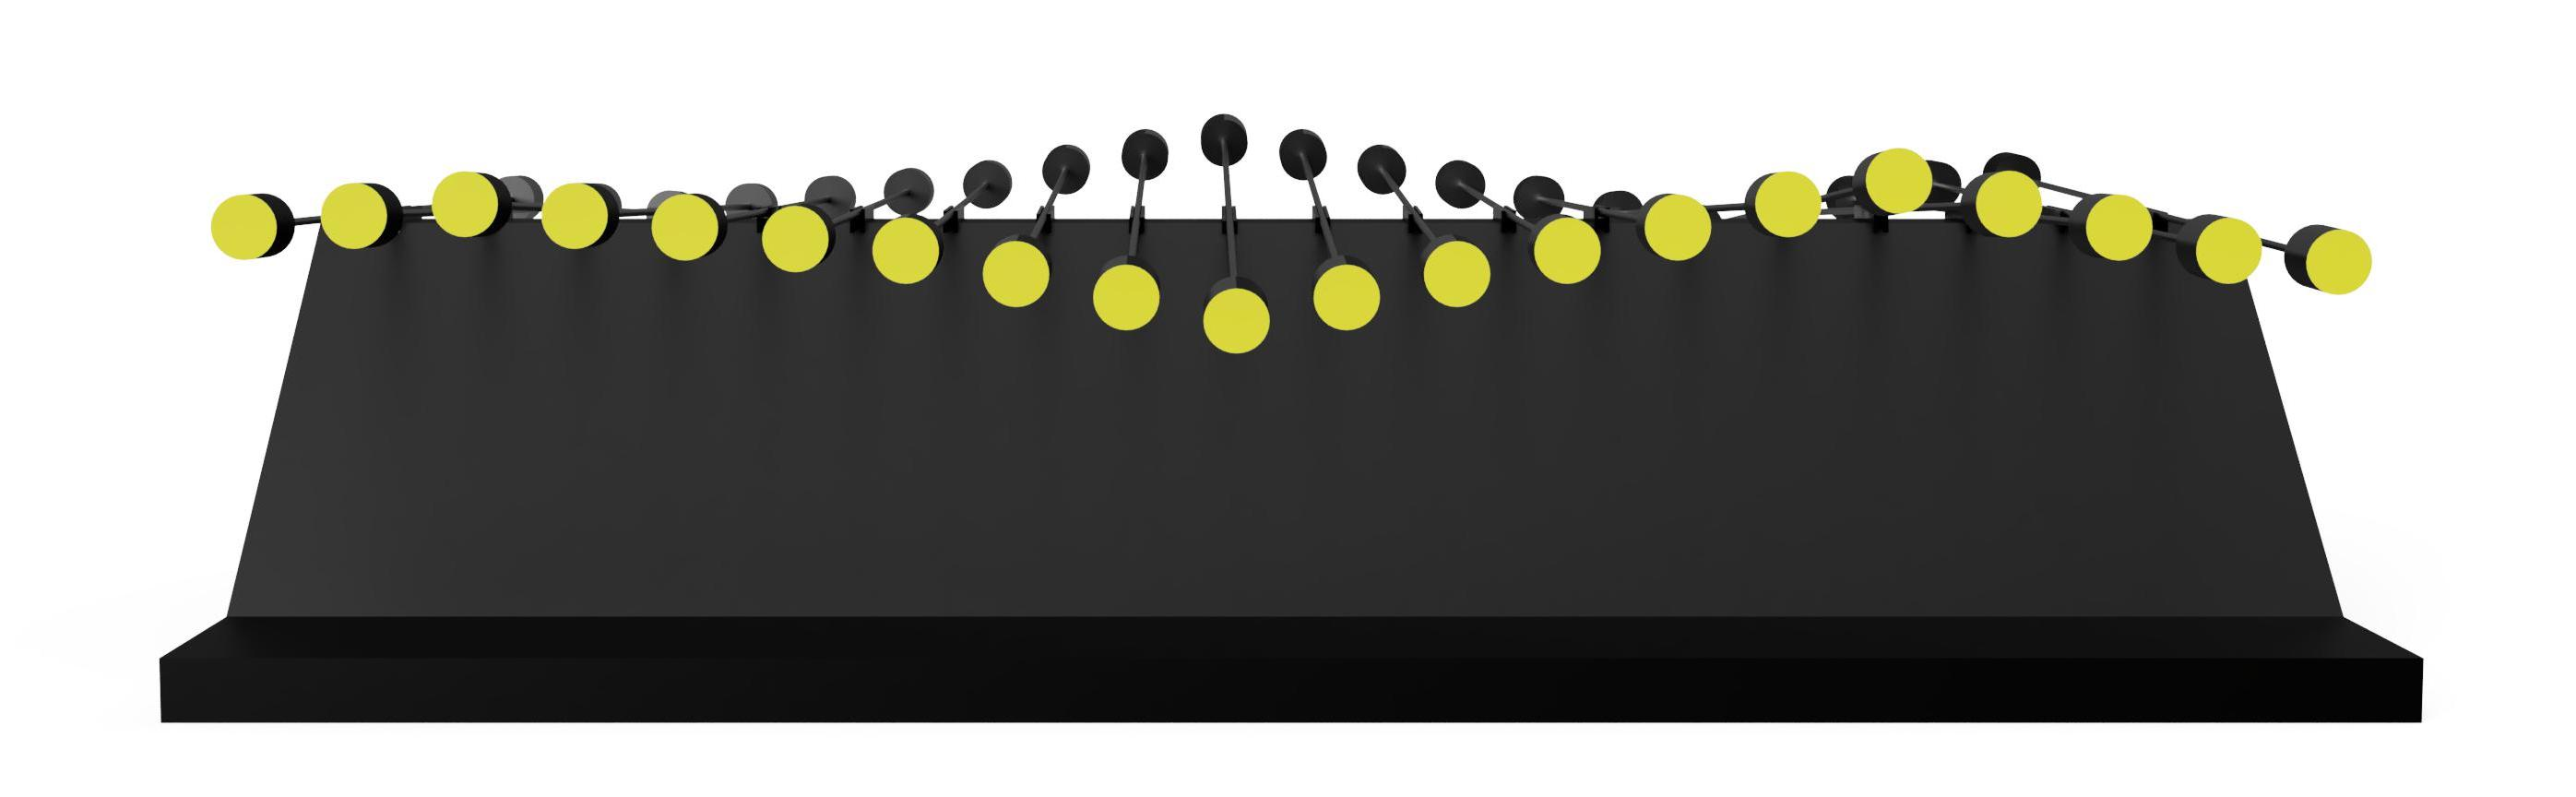
\includegraphics[width=\textwidth]{images/mechanical_wave_machine.jpg}
\end{figure*}

\clearpage

\setcounter{page}{2}                    % make it start with "ii"
\tableofcontents 
\clearpage                       % Print table of contents

\section{Introduction} 
Mass is the 'stuff' that makes up the whole universe (besides energy). Anything we can touch is made up of mass. In physics, mass is defined as "the quantity of matter which a body contains, as measured by its acceleration under a given force or by the force exerted on it by a gravitational field" [1]. Most of the time we observe Newton's Second Law of Motion, in which the force is equal to a positive valued mass of a body times its acceleration. Accordingly, if you push a body it will accelerate in the direction you're pushing it. This occurs for all natural materials, which, under external stimulation react in phase with the excitation. However, researchers have been able to design materials that will accelerate in the opposite direction of the force applied. Under such conditions, the body has a negative effective mass. Effective mass is defined as: "the mass of something as calculated or inferred from its effect in a particular context; the mass that needs to be assigned to a particle if the usual equations of motion are to hold in a situation where they do not strictly apply" [1]. I will investigate negative effective mass experimentally by employing a mechanical wave machine. This wave machine consists of periodically arranged oscillators. As the system is finite I will be able to detect discrete resonances of the unit at specific frequencies. Resonances are phenomena that occur in mechanics when the frequency of the periodically applied excitation is in harmonic proportion to the natural frequency of the system it acts on. After these resonances the oscillators reacts in the opposite direction relative to the excitation, which will model negative effective mass of the wave machine. To verify my hypothesis the local resonances and the transmission property of the wave machine are observed and explained by Newtown's theory.
 
\clearpage

\section{Fundamentals}\label{Fundamentals}
The mechanical wave machine employed in this investigation consists of periodically arranged oscillators that are each connected to two neighbouring oscillators by a spring with constant $k$. The oscillators are excited by a periodic external force, $F_{\rm ext}(t)$. In the sections below, I will introduce the theoretical description of a simple driven harmonic oscillator, a mass with a hidden internal oscillator and a chain of coupled oscillators.

\subsection{Simple Harmonic Oscillator}  
A simple harmonic oscillator can be realised by a mass $m$ coupled via a spring with spring constant $k$ to a wall. The mass shall slide without friction along the ground. The wall can be moved by an external force $F_{\rm ext}(t)$ (see Fig \ref{fig:SHO}).

\begin{figure}[hbt]
  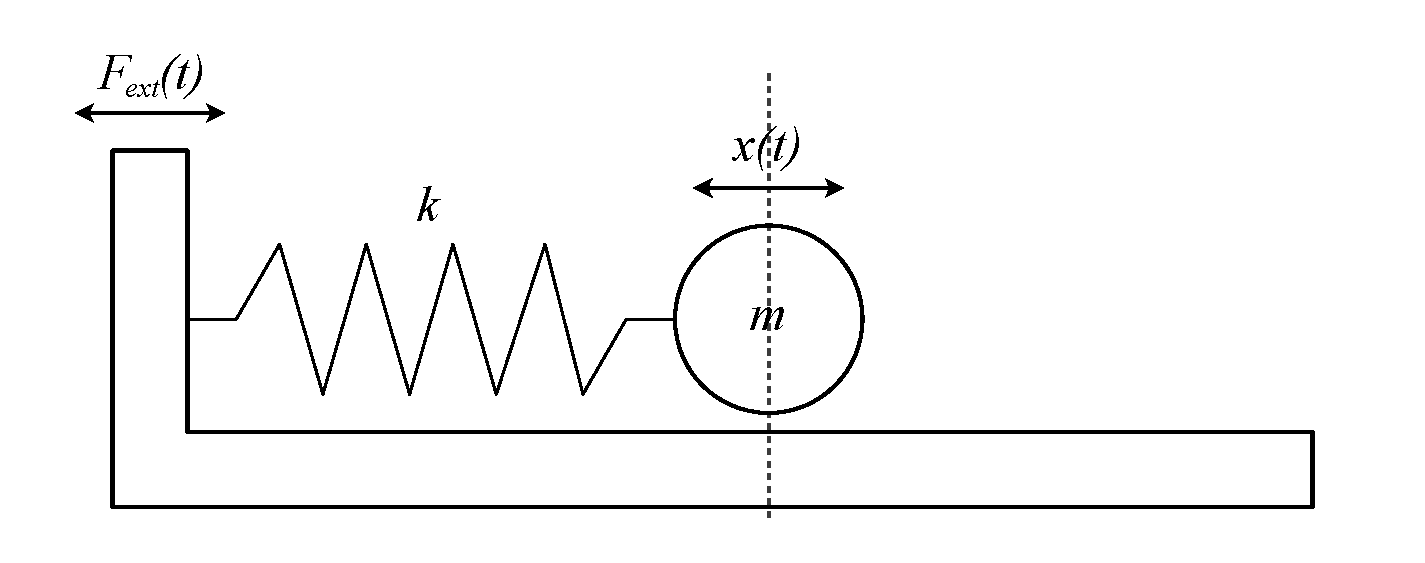
\includegraphics[width=\columnwidth]{fundamentals/simple_harmonic_oscillator.pdf}
  \caption{Model of a simple harmonic oscillator without friction, exposed to an external excitation}\label{fig:SHO}
\end{figure}

The restoring force for such a spring is given by Hooke's law which states that $F_{\rm spring}=~-kx$. The  equation is rewritten as
\begin{equation}\label{eq:diff_eq}
    \frac{d^2 x}{dt^2}=-\frac{k}{m}x =-\omega_{0}^{2}x
\end{equation}
Thus, the solution of this differential equation is a function involving a {\it sine} or {\it cosine} function and can be written in a complex form using Eulers formula. For the initial conditions $x(t=0)=x_0$ and the velocity of the mass $\dot{x}(t)=0$ I find
\begin{equation}\label{eq:3}
x(t)= x_0 e^{-i\omega_0 t}
\end{equation}
If the oscillator is excited with a periodic external force $F_{\rm ext}(t)$
\begin{equation}\label{eq:4}
  F_{\rm ext}(t)=F_{0}e^{-i\omega t}
\end{equation}
I can write down the sum of all of the acting forces in the system of such an oscillator
\begin{equation}\label{eq:5}
F(t)=m\left(-\omega^{2} x \right)=F_{\rm spring}+F_{\rm external}= -\omega^{2}_0mx + F_0e^{-i\omega t}
\end{equation}
This  equation is solved by substituting  $x(t)=x_0 e^{-i\omega t+\phi}$ as the mass will now oscillate with the same frequency of the exciting force. One can then find the amplitude of the oscillation $x_{0}$ as a function of the excitation frequency. 
\begin{equation}\label{eq:7}
  x_0=\frac{F_0}{m(\omega_0^2 - \omega^2)}
\end{equation}

Figure 2 illustrates that eq.~\ref{eq:7} has a singularity at the resonance  $\omega_0 = \omega$.  When $\omega > \omega_0$ the amplitude becomes negative as the external excitation of the oscillator and the oscillation itself are acting in opposite directions ($\phi=\pi$). For $\omega < \omega_0$ the phase angle $\phi=0$.

\begin{figure}[hbt]
  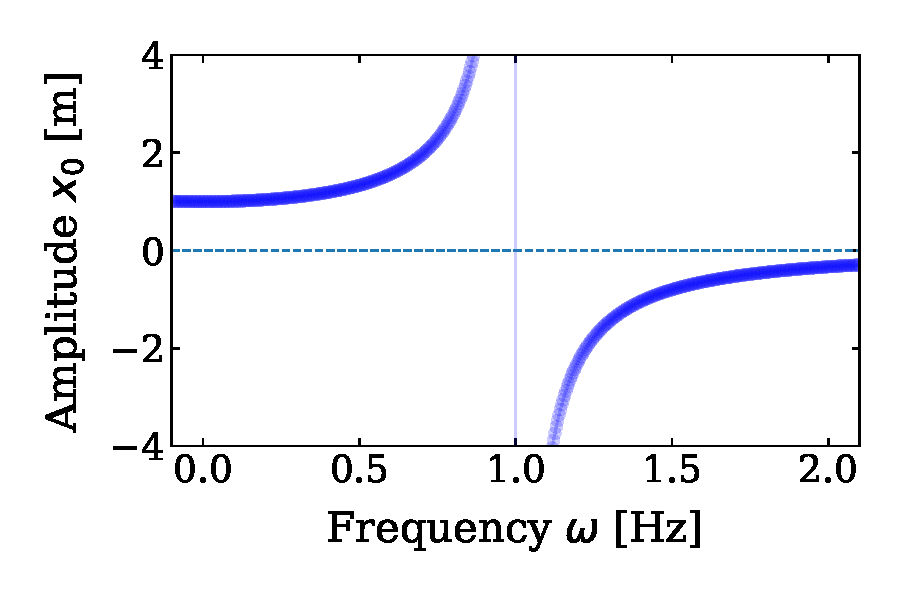
\includegraphics[width=0.5\columnwidth]{fundamentals/driven_harmonic_oscillator}
  \caption{The graph shows eq.\ref{eq:7} when plotted. For simplification arbitrary values were used for $F_0$, $m$ and $\omega_0$ ($F_0=1\, N$, $m = 1 \,kg$, $\omega_0 = 1\, Hz$) to the show the relationship between amplitude $x_0$ and frequency $\omega$.}
\end{figure}


\subsection{Mass with an internal oscillator}
For my experiments I modified the mass $m$ of the oscillator described above. The mass of the new oscillator comprises an internal oscillator inside a larger object with the mass $M_{0}$.
\begin{figure}[hbt]
  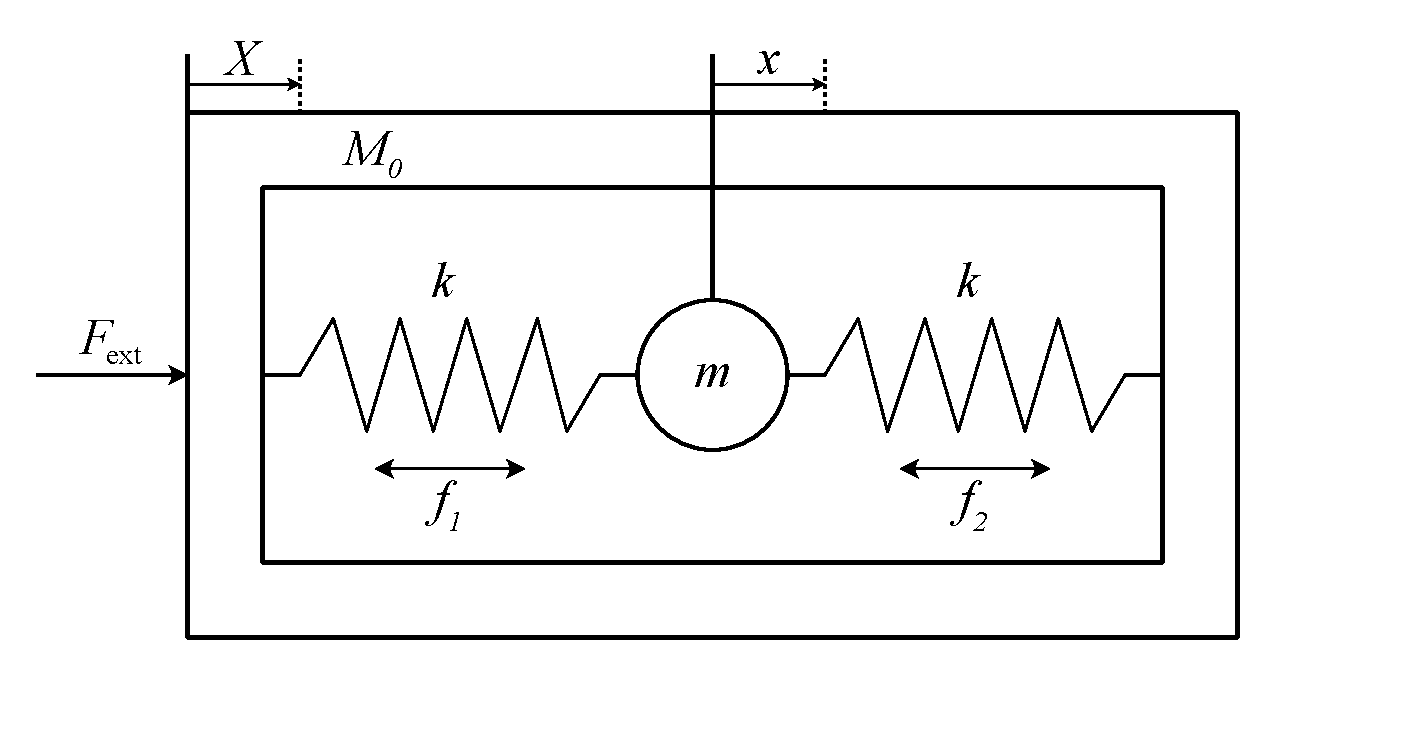
\includegraphics[width=0.7\columnwidth]{fundamentals/oscillator_with_internal_degree_of_freedom.pdf}
  \caption{Model of an oscillator with internal degree of freedom}
\end{figure}
The basic unit is shown in Figure 3. A rigid bar of mass $M_0$ has a cavity to connect to a rigid sphere of mass $m$ by two massless elastic springs with equal constant $k$. The bar together with the internal sphere and springs is equivalent to a solid object with an effective mass of $M_{\rm eff}$. The force of the periodic external excitation is given by the equation, 
\begin{equation}\label{eq:8}
	F_{\rm ext} = \hat{F} e^{-i\omega t}
\end{equation}
where $\hat{F}$ is the amplitude of the excitation. The periodic restoring forces acting on the sphere $m$ are $f_1$ and $f_2$. The amplitude of the restoring forces is defined by $\hat{f_1},\hat{f_2}$. I can write the forces as:
\begin{equation}\label{eq:9}
	f_1 = \hat{f_1} e^{-i\omega t}	
\end{equation}
\begin{equation}\label{eq:10}
	f_2 = \hat{f_2} e^{-i\omega t}	
\end{equation}
The velocity of the bar and the sphere is derived using the displacement $X$ and $x$ respectively. The first derivative of the displacement with respect to time is equal to the velocity: 
\begin{equation}\label{eq:11}
	\hat{V} = -i\omega X	
\end{equation}
\begin{equation}\label{eq:12}
	\hat{v} = -i\omega x
\end{equation}
The force of the external excitation is a sum of the force exerted by the bar and the sphere. The force of  the sphere can be rewritten as the difference between the forces acting on it from the springs. I can therefore note two relationships:
\begin{equation}\label{eq:13}
	\hat{F} = -i\omega M_0 \hat{V} + \left(\hat{f_1}-\hat{f_2}\right) = -i\omega \left(M_0\hat{V} + m\hat{v} \right)
\end{equation}
Both springs have an equal spring constant k and have the same periodicity but act out of phase to each other by $\pi$. Hence, $f_1$ is the negative of $f_2$. The difference between the displacement from equilibrium of the bar, $X$, and the sphere, $x$, is the total displacement of the sphere. The total displacement multiplied by the spring constant $k$ yields the force amplitude $\hat{f}_1$:
\begin{equation}\label{eq:14}
	{\hat f_1} = -{\hat f_2} = k\left(X-x\right)
\end{equation}
When examining eq. \ref{eq:13} it is obvious that the difference between $\hat f_1$ and $\hat f_2$  is equal to first time derivative of the momentum of the sphere (eq.~\ref{eq:15}).
\begin{equation} \label{eq:15}
	\hat f_1 - \hat f_2= 2k\left(X-x\right)= -i\omega(m\hat v)
\end{equation}
I can employ eq. \ref{eq:15} and expand $\hat v$ to its constituents such that 
\begin{equation}\label{eq:16}
		2kX -2kx = -\omega^2 mx
\end{equation}
When simplified I obtain the relationship between the instantaneous velocity, $\hat v$, of the sphere and the instantaneous velocity, $\hat V$ of the bar
\begin{equation}\label{eq:17}
	\hat{v} =\frac{2k}{2k -m\omega ^2}\hat{V}
\end{equation}
I can use eq. \ref{eq:17} and substitute it into eq. \ref{eq:13}
\begin{equation}\label{eq:18}
	\hat{F} = -i\omega\left(M_0	\hat{V} + m\frac{2k}{2k -m\omega ^2}\hat{V}\right)
\end{equation}
The effective mass $M_{\rm eff}$ is defined as the total force divided by the acceleration. This leads to 
\begin{equation}\label{eq:19}
	M_{\rm eff} = M_0 + \frac{2km}{2k -m\omega ^2}.
\end{equation}
The resonance frequency of the internal oscillator is expressed by $\omega_0 = \sqrt{2k/m}$. When substituting this relation I obtain
\begin{equation}\label{eq:20}
 M_{\rm eff} =	M_0 + \frac{m \omega_0^2}{\omega_0^2 -\omega ^2}
\end{equation} 
Equation eq. \ref{eq:20} shows that the effective mass $M_{\rm eff}$ can be negative in the frequency range from $\omega_0$ to $\omega_0 \sqrt{(M_0 + m)/ M_0}.$ The negativity of the effective mass comes from the negative momentum of the sphere, since it moves in the opposite direction relative to the bar after resonance. 
\begin{figure}[hbt]
  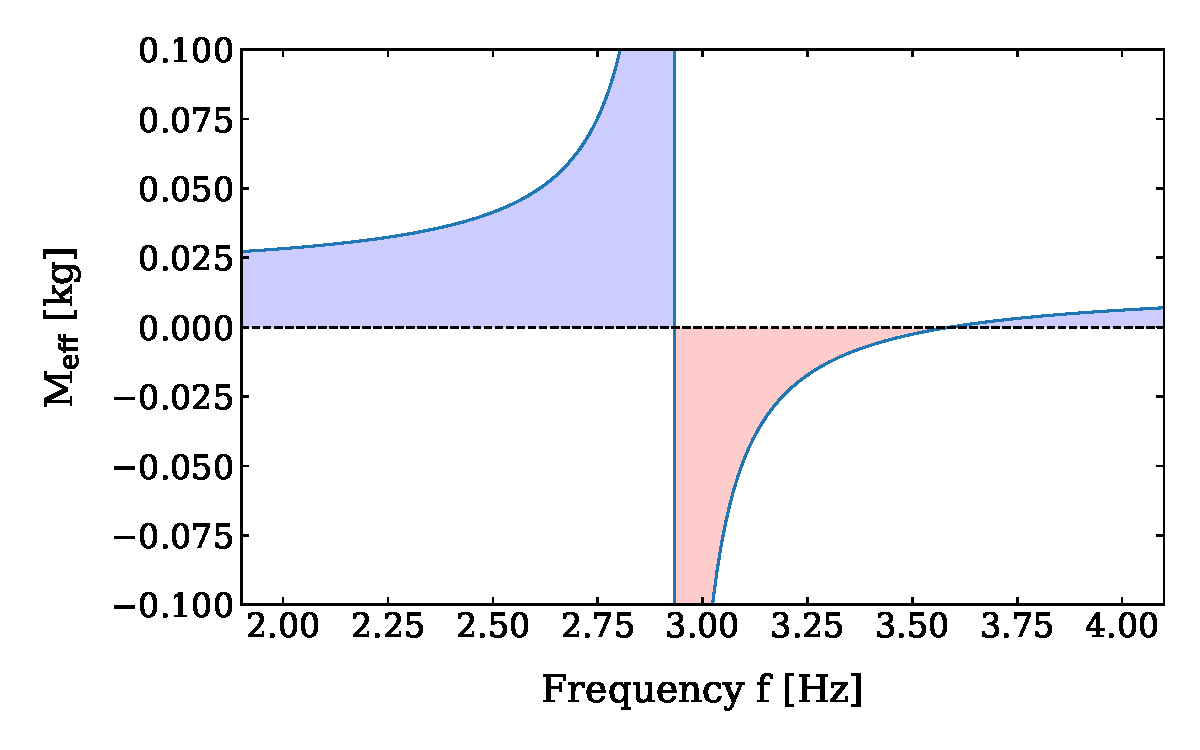
\includegraphics[width=0.7\columnwidth]{fundamentals/effective_mass.pdf}
  \caption{Effective mass according to eq. \ref{eq:20} with $m=0.0073 kg$, $M_{0}=0.0146\, g$ and $\omega_0=2\pi f_{0}=18.52\,{\rm Hz}$. The red shaded area indicates the frequency region in which the effective mass of the oscillator is negative.}
\end{figure}
Figure 4 illustrates that when examining an object with internal oscillator by employing Newton's theory I obtain a frequency range in which the effective mass of the oscillator appears to be negative.

    From eq. \ref{eq:17} I can also determine the transmission properties of the unit, in terms of the amplitude ratio between the sphere given by $x$ and the bar given by $X$. The relationship between $x$ and $X$ can be mathematically expressed as
    \begin{equation} \label{eq:ratio}
        \frac{x}{X} = \frac{2k_{\rm eff}}{2k_{\rm eff} - m\omega^2}
    \end{equation}
I obtain a singularity at $\omega = \omega_0$. As $\omega$ approaches $\omega_0$ the amplitude of $x$ enlarges. After the resonance the amplitude ratio becomes negative and then approaches zero. 
\subsection{Chain of Coupled Oscillators - Waves}\label{sec:coupled:waves}
The negative effective mass has several consequences for a chain of oscillators where the units with $M_{\rm eff}$ as described before are coupled with equal springs of constant $k$, as shown in Figure 5. 
\begin{figure}[hbt]
  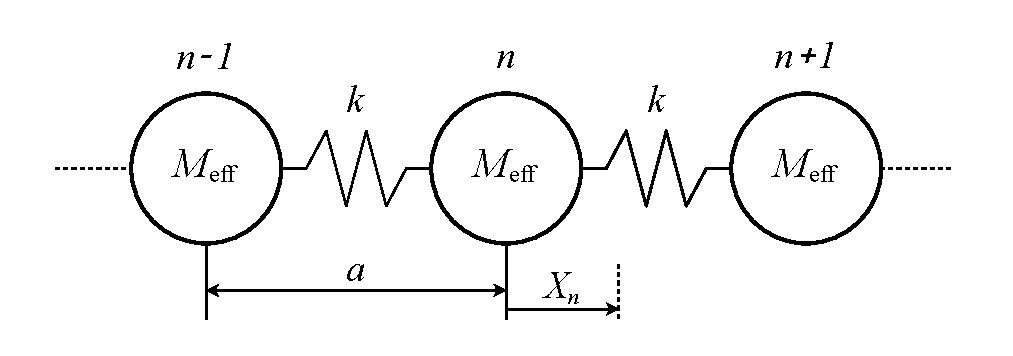
\includegraphics[width=0.8\columnwidth]{fundamentals/chain_of_oscillators.pdf}
  \caption{An infinite periodic mass-spring system}
\end{figure}
The negative effective mass will change the so-called dispersion relation and the transmission of waves through the chain. The dispersion relation refers to the mathematical relationship between the wavenumber $q$ and the frequency $\omega$ and can be obtained analytically. The spacing between each unit is assumed to be $a$. From Newton's law of motion, the force on the $n$th mass proves to be the following equation, where $X_n$ is the displacement of the $n$th unit.
\begin{equation}\label{eq:21}
	F_{n} = k (X_{n+1} - X_n) + k(X_{n-1} - X_n)
\end{equation}
For a harmonic system of oscillators this leads to
\begin{equation}\label{eq:22}
-\omega^2 M_{\rm eff} X_n = k \left(X_{n+1} + X_{n-1} - 2X_n \right)	
\end{equation}
According to the Bloch theorem and periodic boundary conditions, the displacement of each unit can be represented by $X_n = Ae^{i(qna - \omega t)}$, where $q$ is the Bloch wavenumber.  Inserting $X_n$ into eq. \ref{eq:22} I find:
\begin{equation}\label{eq:23}
	-\omega^2 M_{\rm eff} e^{i(qna - \omega t)} = k\left(e^{i(q(n+1)a - \omega t)} + e^{i(q(n-1)a - \omega t)} - 2e^{i(qna - \omega t)}\right)	
\end{equation}
\begin{equation}\label{eq:24}
	-\omega^2 M_{\rm eff} = k\left(e^{iqa} + e^{-iqa} - 2\right)
\end{equation}
\begin{equation}\label{eq:25}
	\omega^2 M_{\rm eff} = 4k\sin^2\left(\frac{qa}{2} \right)
\end{equation}
From eq. \ref{eq:25} I get the dispersion relation for an infinite periodic system. When the effective mass $M_{\rm eff}$ becomes negative, the $\sin^{2}$ has to yield an imaginary number, which is only possible for an imaginary wavenumber $q=i\kappa$ ($\kappa$ is a real number). In this case the exponential factor in the Bloch wave, i.e. $e^{-\kappa n a}$ will become a real valued and the amplitude of the oscillations will decay exponentially with the distance from the excitation source. Thus no waves are supported in this negative effective mass region by the chain. This region will correspond to a so-called band gap in the dispersion relation eq. \ref{eq:25}. This is a signature of the negative mass I want to observe in my experiments.

\section{Experimental Setup}
\subsection{Equipment List and Experimental Setup}
\subsubsection{Equipment List}
\begin{enumerate}
	\item Mechanical Wave Machine (Length = 40 cm)
	\item USB camera
	\item Computer
	\item Frequency Generator
	\item Actuator
	\item Pincer (to connect the actuator to the first lever of the wave machine)
	\item 3D-printed brackets 
\end{enumerate}

\subsubsection{Experimental Setup}  \label{sec:section3}
To verify the frequency-dependent effective mass of the unit analysed in the previous section, I conducted an experiment of the 2D mass-spring system, for which a mechanical wave machine was employed. The wave machine is different to the model analysed previously.
	Section 5.1 discusses its equivalence to the described theory.
\begin{figure}[hbt]
  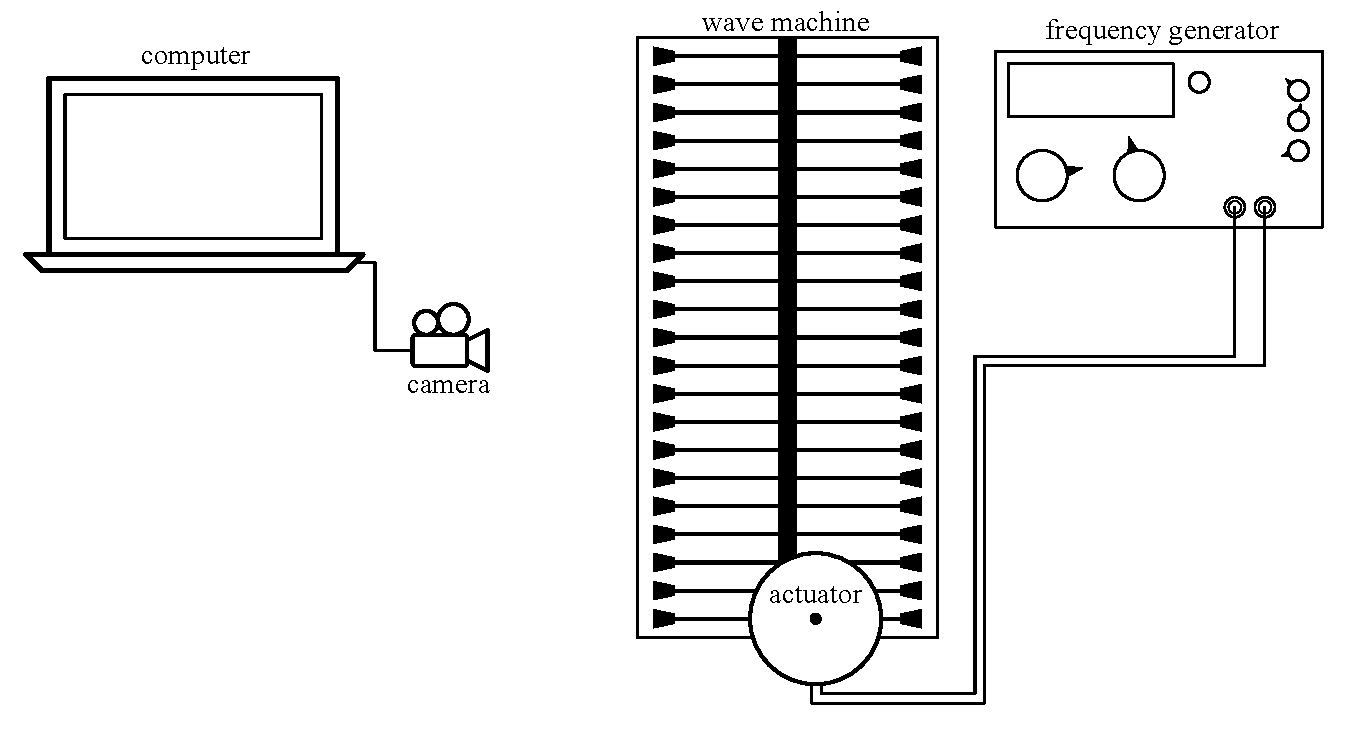
\includegraphics[width=.8\columnwidth]{experimental_setup/experimental_setup_sketch}
  \caption{Scheme of the experimental setup from the top view}
\end{figure}
\begin{figure}[hbt]
  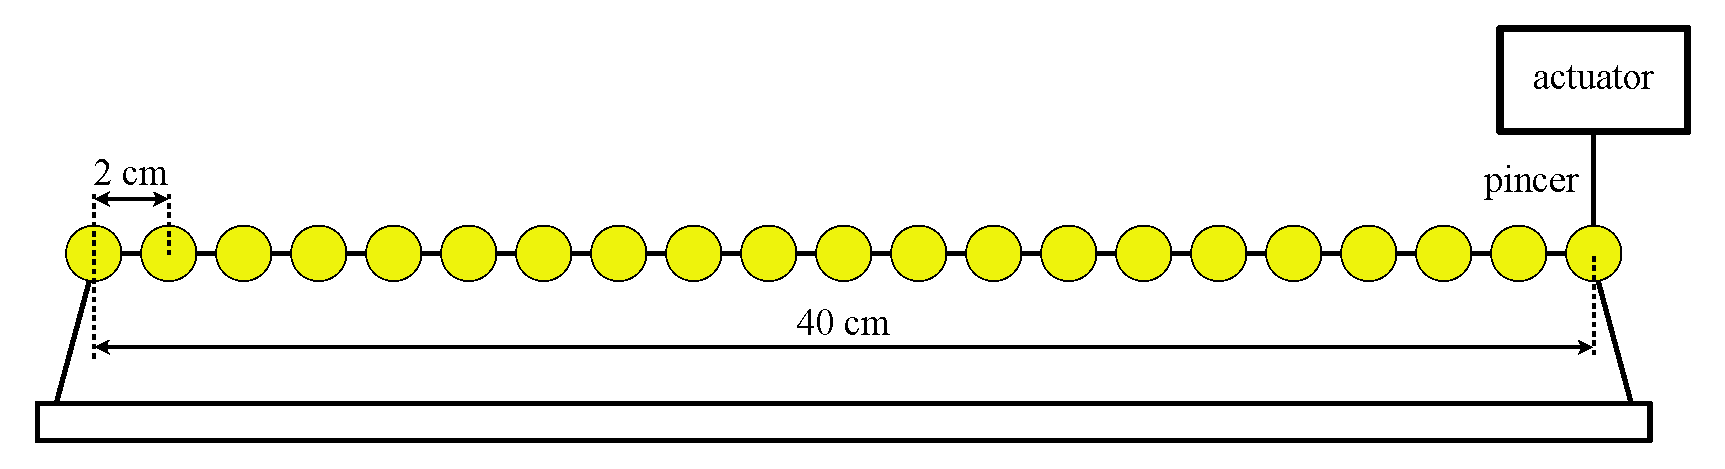
\includegraphics[width=.8\columnwidth]{experimental_setup/experimental_setup_sketch_side}
  \caption{Scheme of the wave machine from the side}
\end{figure}

Figures 6 and 7 display the experimental setup. The wave machine has a length of $40\, {\rm cm}$ and consists of 21 levers marked by a yellow dot (Figure 7). The distance between the centres of each lever is $a=2\, {\rm cm}$. The actuator is connected by a pincer to the first lever and is driven by a frequency generator. The motion of the levers was detected by a USB camera. The camera captures 30 fps ($0.033 \, {\rm s}$ per frame). At each frequency a movie of a total length of $15\,{\rm s}$ was recorded (450 frames in total). The data was stored on the computer and analysed through a self-written python code. 

\subsection{Measurement Configurations}
The effect of a periodic excitation on the wave machine was investigated under three different configurations. Therefore the wave machine was manipulated with 3D-printed brackets. In all cases, the excitation is perpendicular to the connection of the levers.

\paragraph{C1: Single mass with an internal degree of freedom.} The first configuration (C1) employs a bracket to form a single mass with an internal oscillator out of three levers. Out of the three levers the first and last lever are fixed together by the bracket. The middle lever is free to move on its own and resembles the internal oscillator. Figure \ref{fig:figure9} sketches the arrangement of the configuration C1.
\begin{figure}[hbt]	
  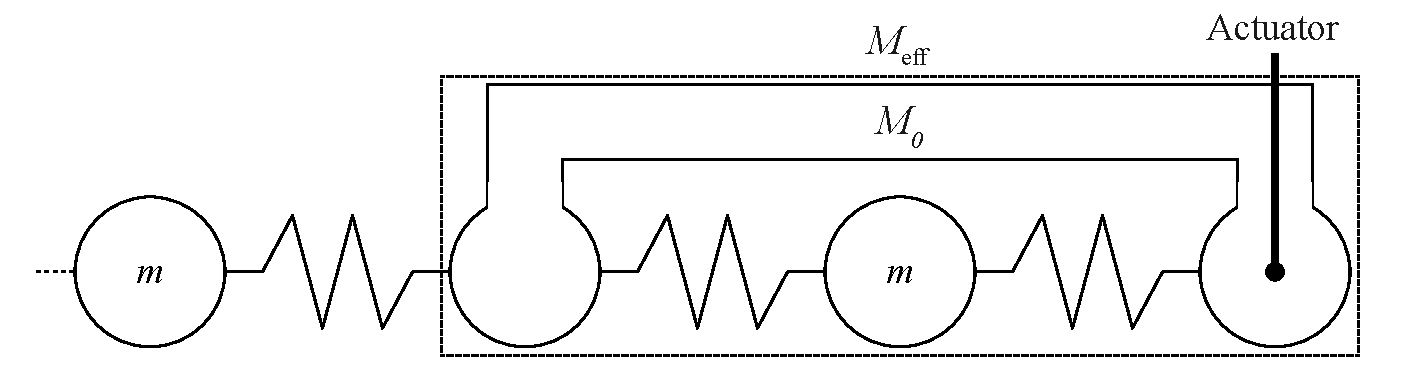
\includegraphics[width=.7\columnwidth]{configurations/condition3.pdf}
  \caption{Scheme of the wave machine for configuration C1, as a single mass with an internal degree of freedom. The unit has the effective mass $M_{\rm eff}$ consists of $M_0$ and the internal mass $m$. $M_0$ is equal to the mass $2m$.}\label{fig:figure9}
\end{figure}
\paragraph{C2: Simple chain of oscillators}In the second configuration C2 the wave machine is left in its original state and the levers are only connected to each other by springs (see Figure 9).
\begin{figure}[h!]	
  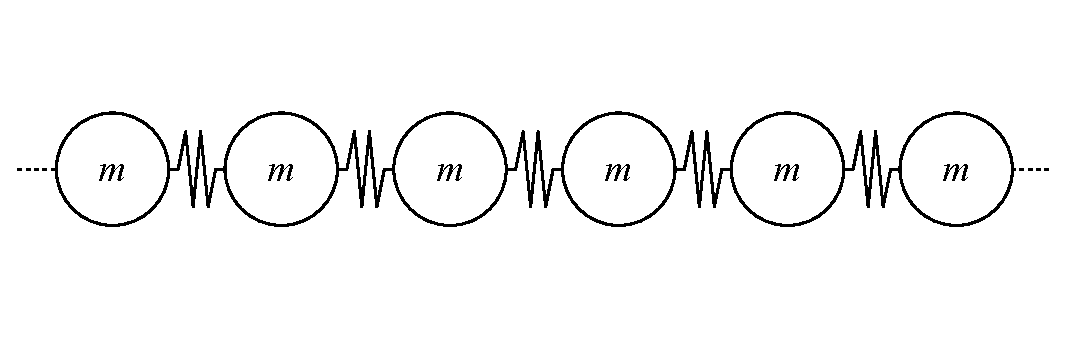
\includegraphics[width=.7\columnwidth]{configurations/condition1.pdf}
  \caption{Scheme of the wave machine for configuration C2, as a simple chain of masses. Each mass $m$ is representative of a single lever, which is connected to neighbouring levers by a spring with constant k.}
\end{figure}

\paragraph{C3: Chain of masses with an internal oscillator.}For the third configuration C3 the wave machine was altered through the addition of 3D-printed brackets. Three levers form a single unit, which is connected to the next by springs. Overall, this investigation uses a chain of 7 such units, with a distance of 6 cm between each other.
\begin{figure}[hbt]	
  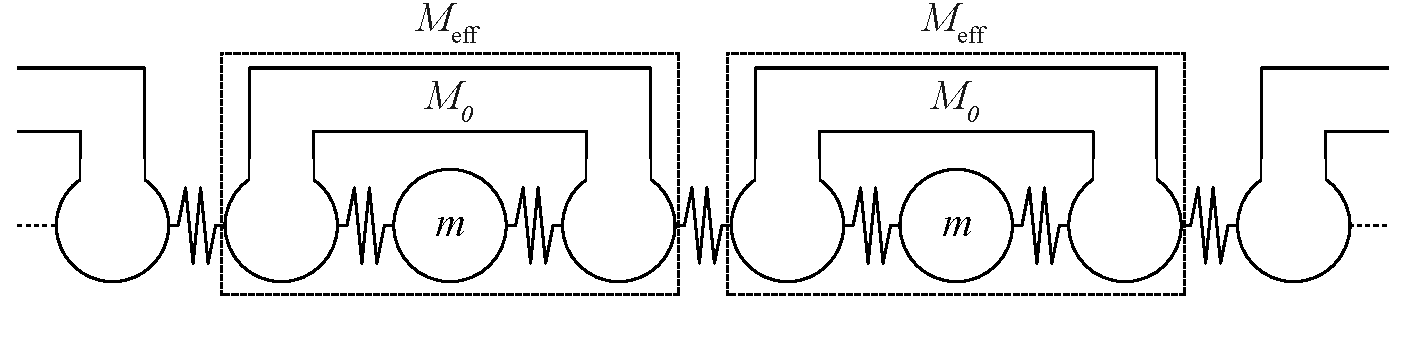
\includegraphics[width=.7\columnwidth]{configurations/condition2.pdf}
  \caption{Scheme of the model for the configuration C3, as a chain of masses with an internal degree of freedom. The unit has the effective mass $M_{\rm eff}$ consists of $M_0$ and the internal mass $m$. $M_0$ is equal to the mass $2m$.} \label{fig:figure8}
\end{figure}

\subsection{Safety Precautions}
Working with technology, like a computer and a frequency generator safety precautions such as current protection are obligatory. Therefore, any liquid was kept away from any technological object such that it will not damage them. In my experiment there are no harmful substance involved, hence, normal safety precautions were taken. 

\section{Data Analysis}\label{sec:section4}
To analyse the motion of each lever, I used a colour tracking procedure developed specifically for this project and written in python (attached to this document). Each recorded frame is analysed as explained below. From this I obtain the horizontal and vertical position of each mass on the lever as a function of time. 

%When analysing a single lever, such as the first or the last, we are able to measure of how much of the initial amplitude is arriving at the end of the chain. We define this amplitude ratio as the transmittance, which is equal to 1 in the case that the last and the first lever have the same amplitude. Besides this we may also access a snapshot of the whole chain at each specific time. This snapshot allows us to identify the wavelength of the wave and thus also the wavenumber associated with it. From this data, we can construct the dispersion relation of the whole system. 

\subsection{Explanation of the Python Software}
\subsubsection{Color Tracking}
The levers were tracked using yellow markers at each lever. Figure \ref{fig:raw} shows a representative image as recorded by the camera. 

\begin{figure}[hbt]
  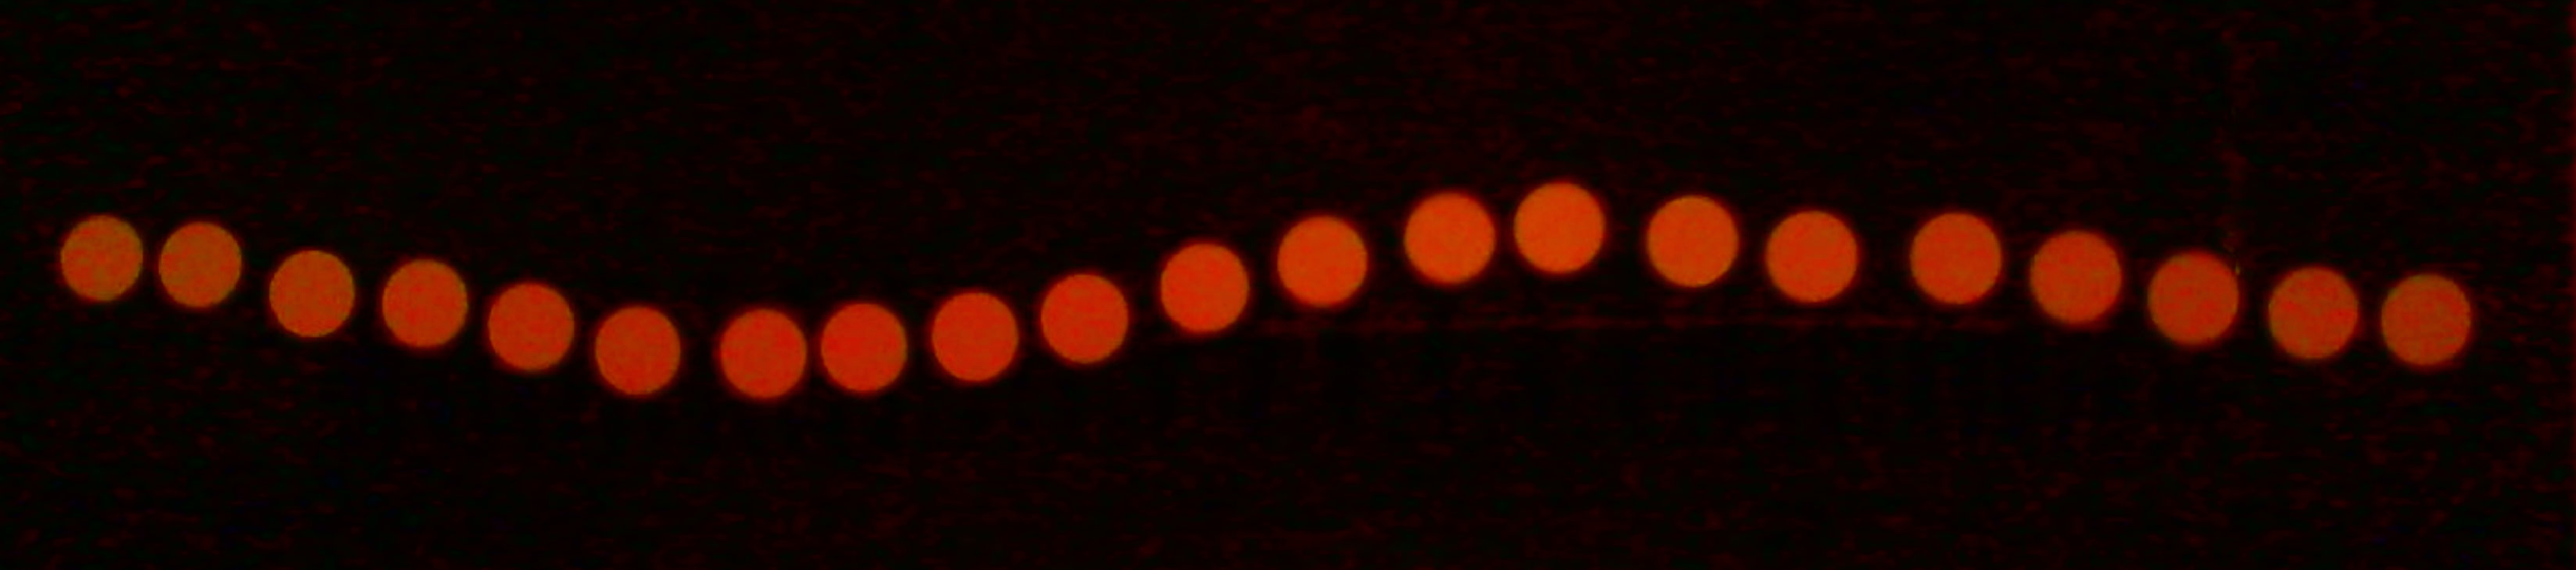
\includegraphics[width=.6\columnwidth]{analysis/data_analysis_sample_frame}
  \caption{Sample image taken from the camera. Each red region represents a lever of the wave machine. The red dots correspond to the yellow markers.}\label{fig:raw}
\end{figure}

The images are imported into the python program. I select only the pixels in a certain color region representing the yellow dots. By this procedure, I achieve a binarization of the image into black or white areas. A sample frame is shown in Figure \ref{fig:binary}.
\begin{figure}[hbt]
  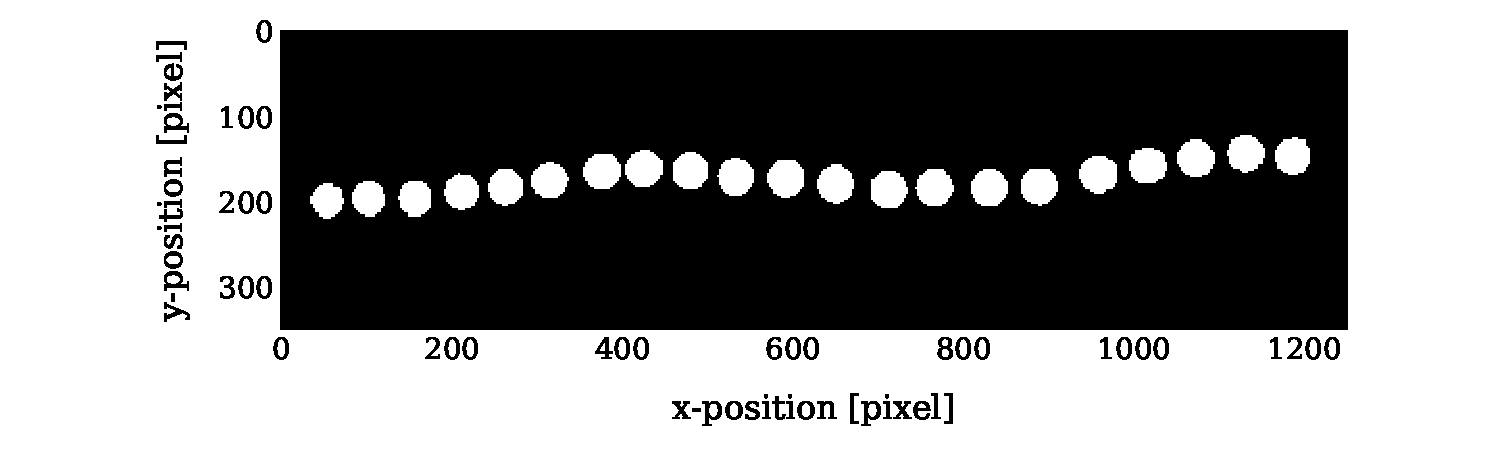
\includegraphics[width=.8\columnwidth]{analysis/colour_channel_adjustment}
  \caption{Sample frame after the binarization of the previous image using a selection of a certain color range.} \label{fig:binary}
\end{figure}
This binarized image can now be used with built-in procedures of the skimage python module to identify the centre positions of the lever masses. I employ the difference of gaussians blob tracking method of skimage, which delivers the positions of each lever [5]. All lever positions in one frame are recorded in a data array and the procedure is repeated for all frames in the recorded movie for each excitation frequency of the wave machine.  The positions are exported to a CSV file for further data analysis. Figure \ref{fig:tracked} illustrates a sample frame after each lever has been properly tracked.
\begin{figure}[hbt]
  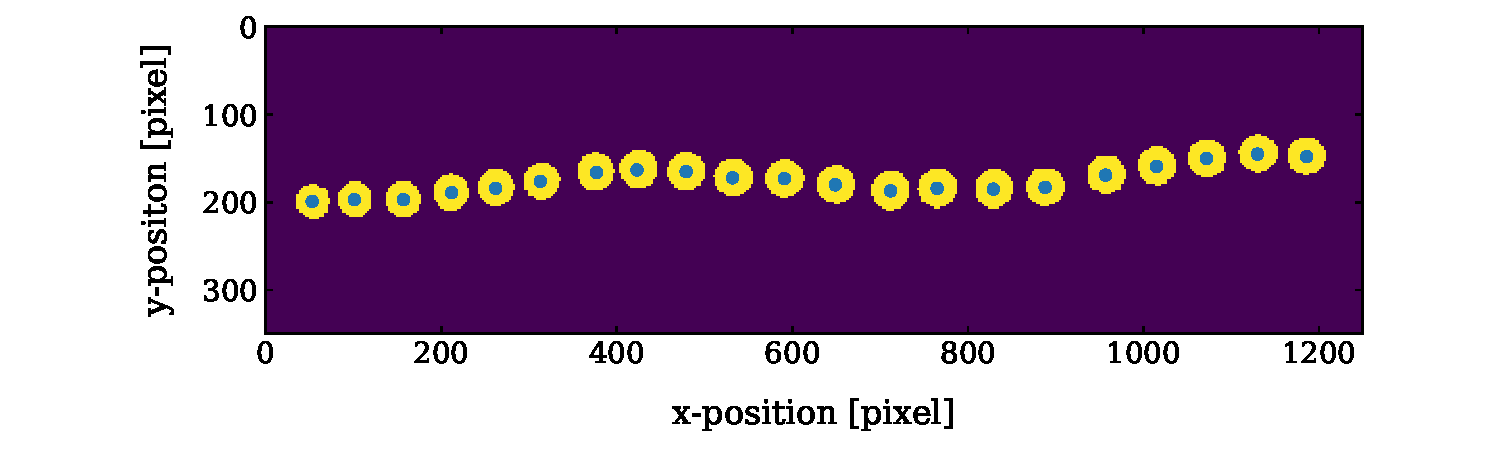
\includegraphics[width=.8\columnwidth]{analysis/blob_tracking}
  \caption{Sample frame after each lever has wavenumber been detected. The dots inside the yellow regions are indicators for the tracked positions of the levers.}\label{fig:tracked}
\end{figure}
\subsubsection{Amplitude ratio}
To determine the amplitude of each lever its positions during all frames are plotted in a single graph (Figure \ref{fig:elongations}).
\begin{figure}[hbt]
  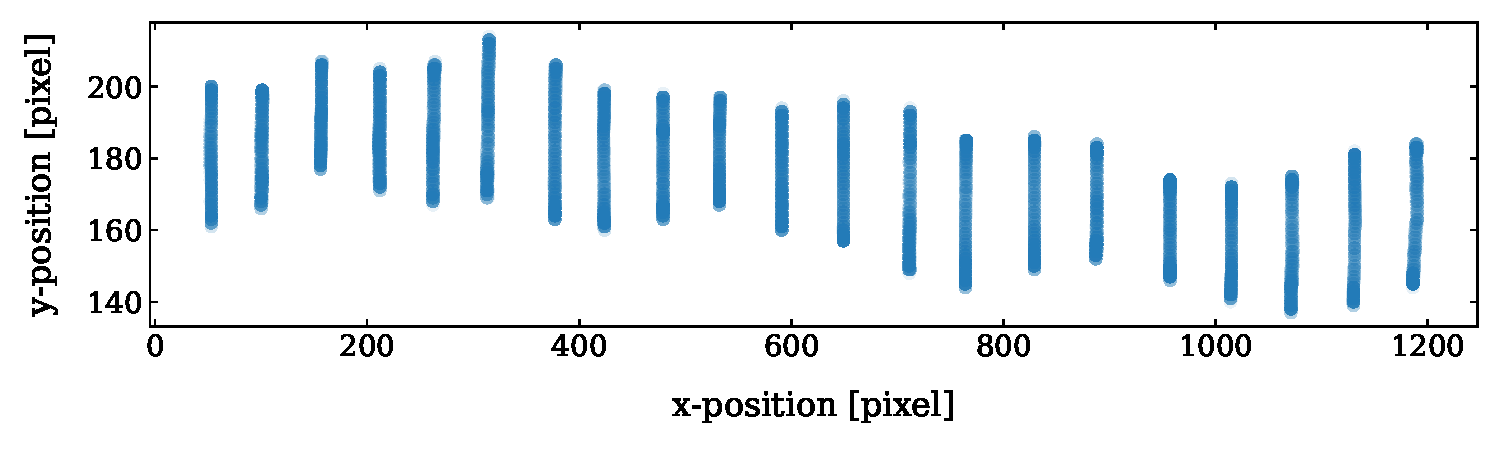
\includegraphics[width=.8\columnwidth]{analysis/amplitude}
  \caption{Plot of elongations for all the frames in the data recording.}\label{fig:elongations}
\end{figure}
From Figure \ref{fig:elongations} I can isolate the tracking of the first (rightmost) and last (leftmost) lever of the wave machine. I then determine the difference between the maximum and the minimum y-position of both corresponding to the total amplitude $X=X_{\rm max}-X_{\rm min}$. This is employed to derive the amplitude ratio $|X_{21}|/|X_1|$ (transmission). This procedure is used for two configurations C2 and C3. In configuration C1 I extracted the amplitude ratio through $|x_{m}|/|X_{M_{0}}|$, which are the displacements of $m$ and $M_0$, respectively.

\subsubsection{Wavelength and wavenumber determination}
To determine the wavelength and wavenumber I converted the distance in pixel to centimeters using the known length of the wave machine. The wavelength and wavenumber are deduced from a single frame, by fitting a sine function ($y(x) = A\sin(qx + \phi) + B$) to the positioning of the detected levers. 
\begin{figure}[hbt]
  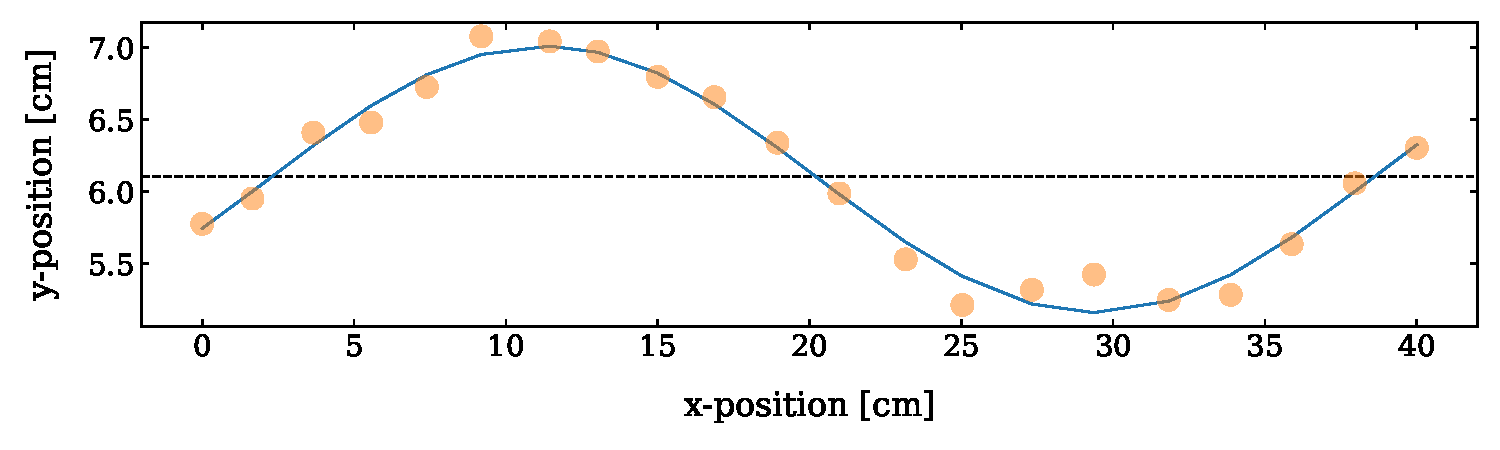
\includegraphics[width=0.8\textwidth]{analysis/wavelength_determination}
  \caption{Sine curve, of the form $y(x) = A\sin(qx + \phi) + B$, modeled to the positioning of the levers. The dotted line represents the equilibrium position}\label{fig:wavelength}
\end{figure}
Figure \ref{fig:wavelength} shows a sample graph. The circles mark the position of each lever and the blue line represents the fitted function. The wavenumber $q$ and the wavelength are related by $q = 2\pi/\lambda$. The parameter $B$ corresponds to an offset of the levers in the vertical direction. The parameter $\phi$  denotes the spatial phase of the wave. 

\section{Results}\label{sec:section5}
\subsection{Equivalence of the wave machine and the oscillator model}\label{sec:results:equivalence}
The theory described in section 2 refers to a model where masses are coupled by springs and create a longitudinal wave with a one dimensional motion. For my investigations, however, I had a wave machine, which is a system of coupled levers which rotate around a central axis (Figure \ref{fig:config}). 
\begin{figure}[hbt]
  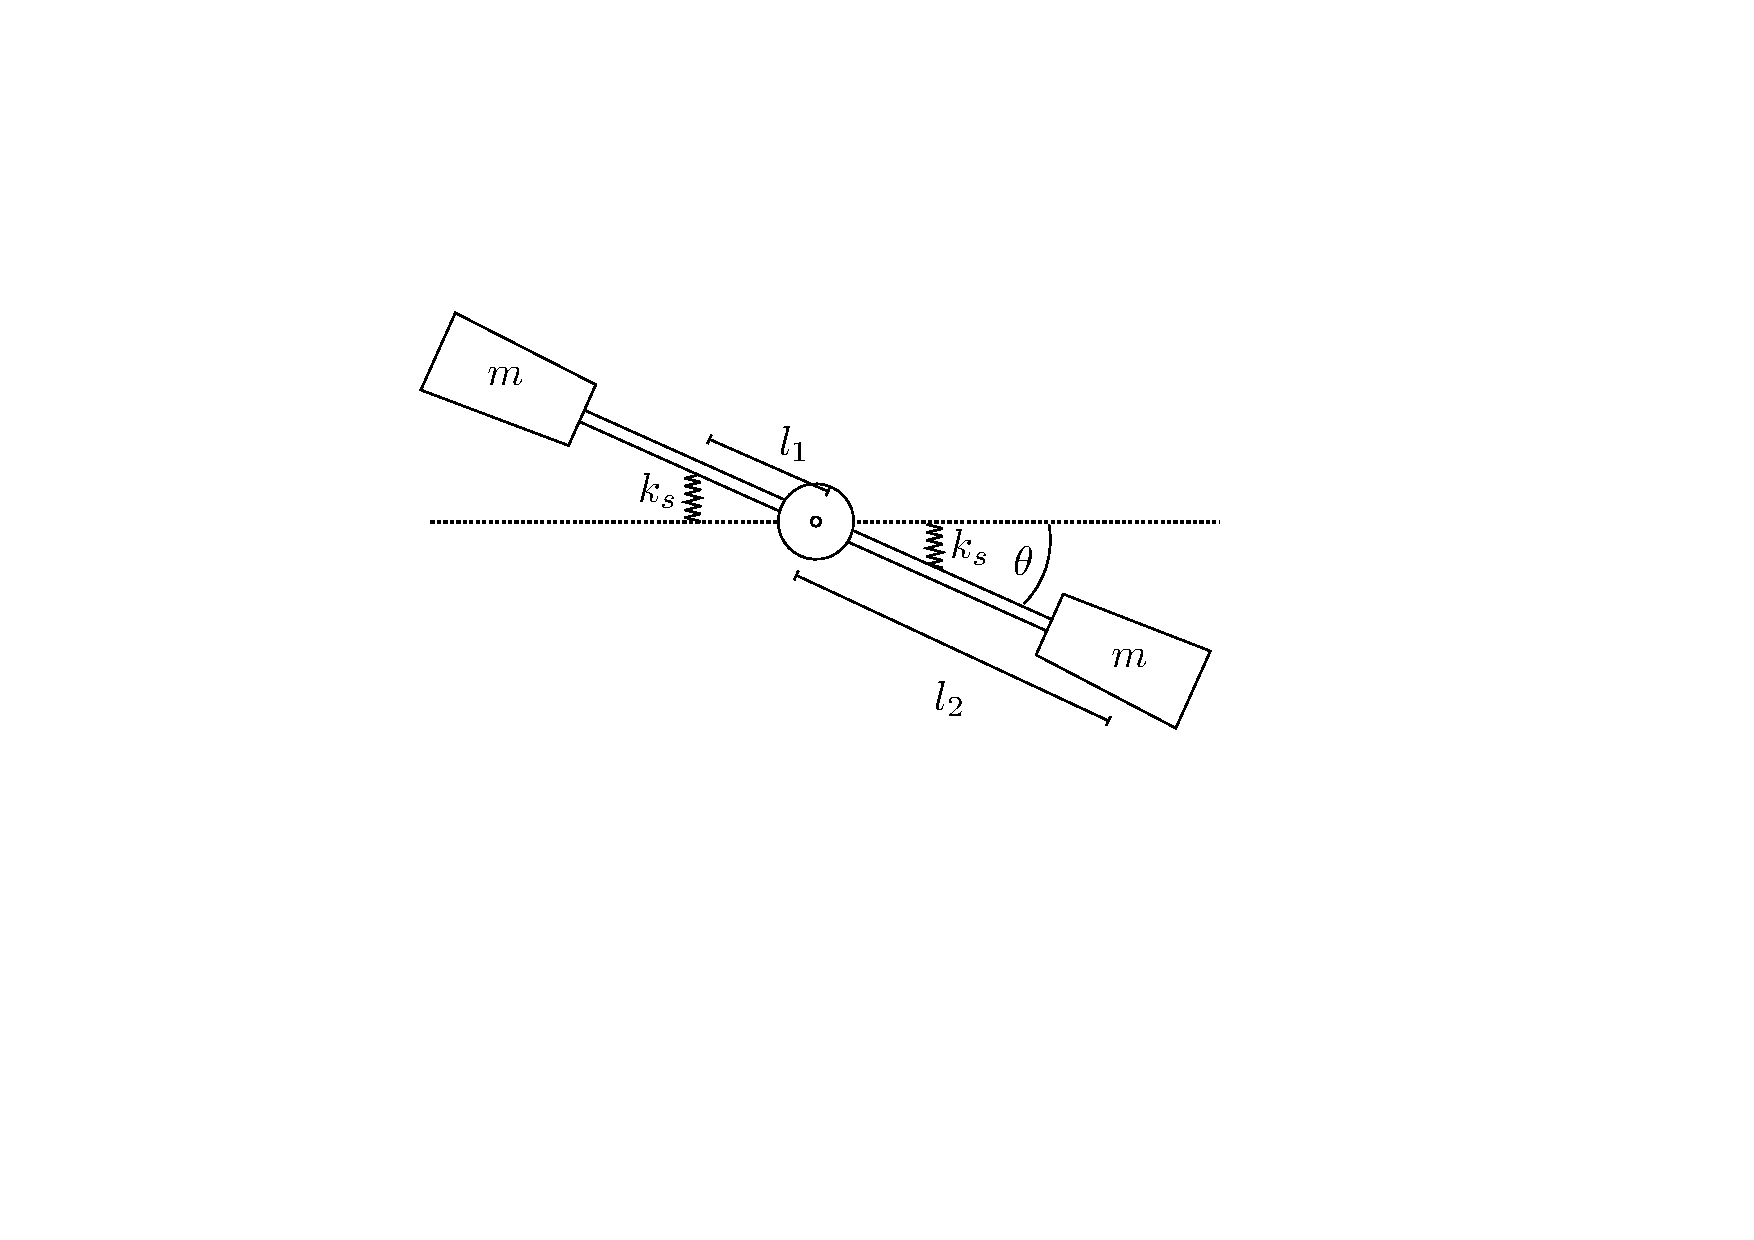
\includegraphics[width=0.5\textwidth]{results/equivalance_new.pdf}
  \caption{Sketch of the configuration of the lever arms in the wave machine. Each of the masses at the end of the levers has a weight of $m=7.3$ g. The spring constant of each spring is $k_s=32.3\, Nm^{-1}$}\label{fig:config}
\end{figure}

\begin{figure}[hbt]
  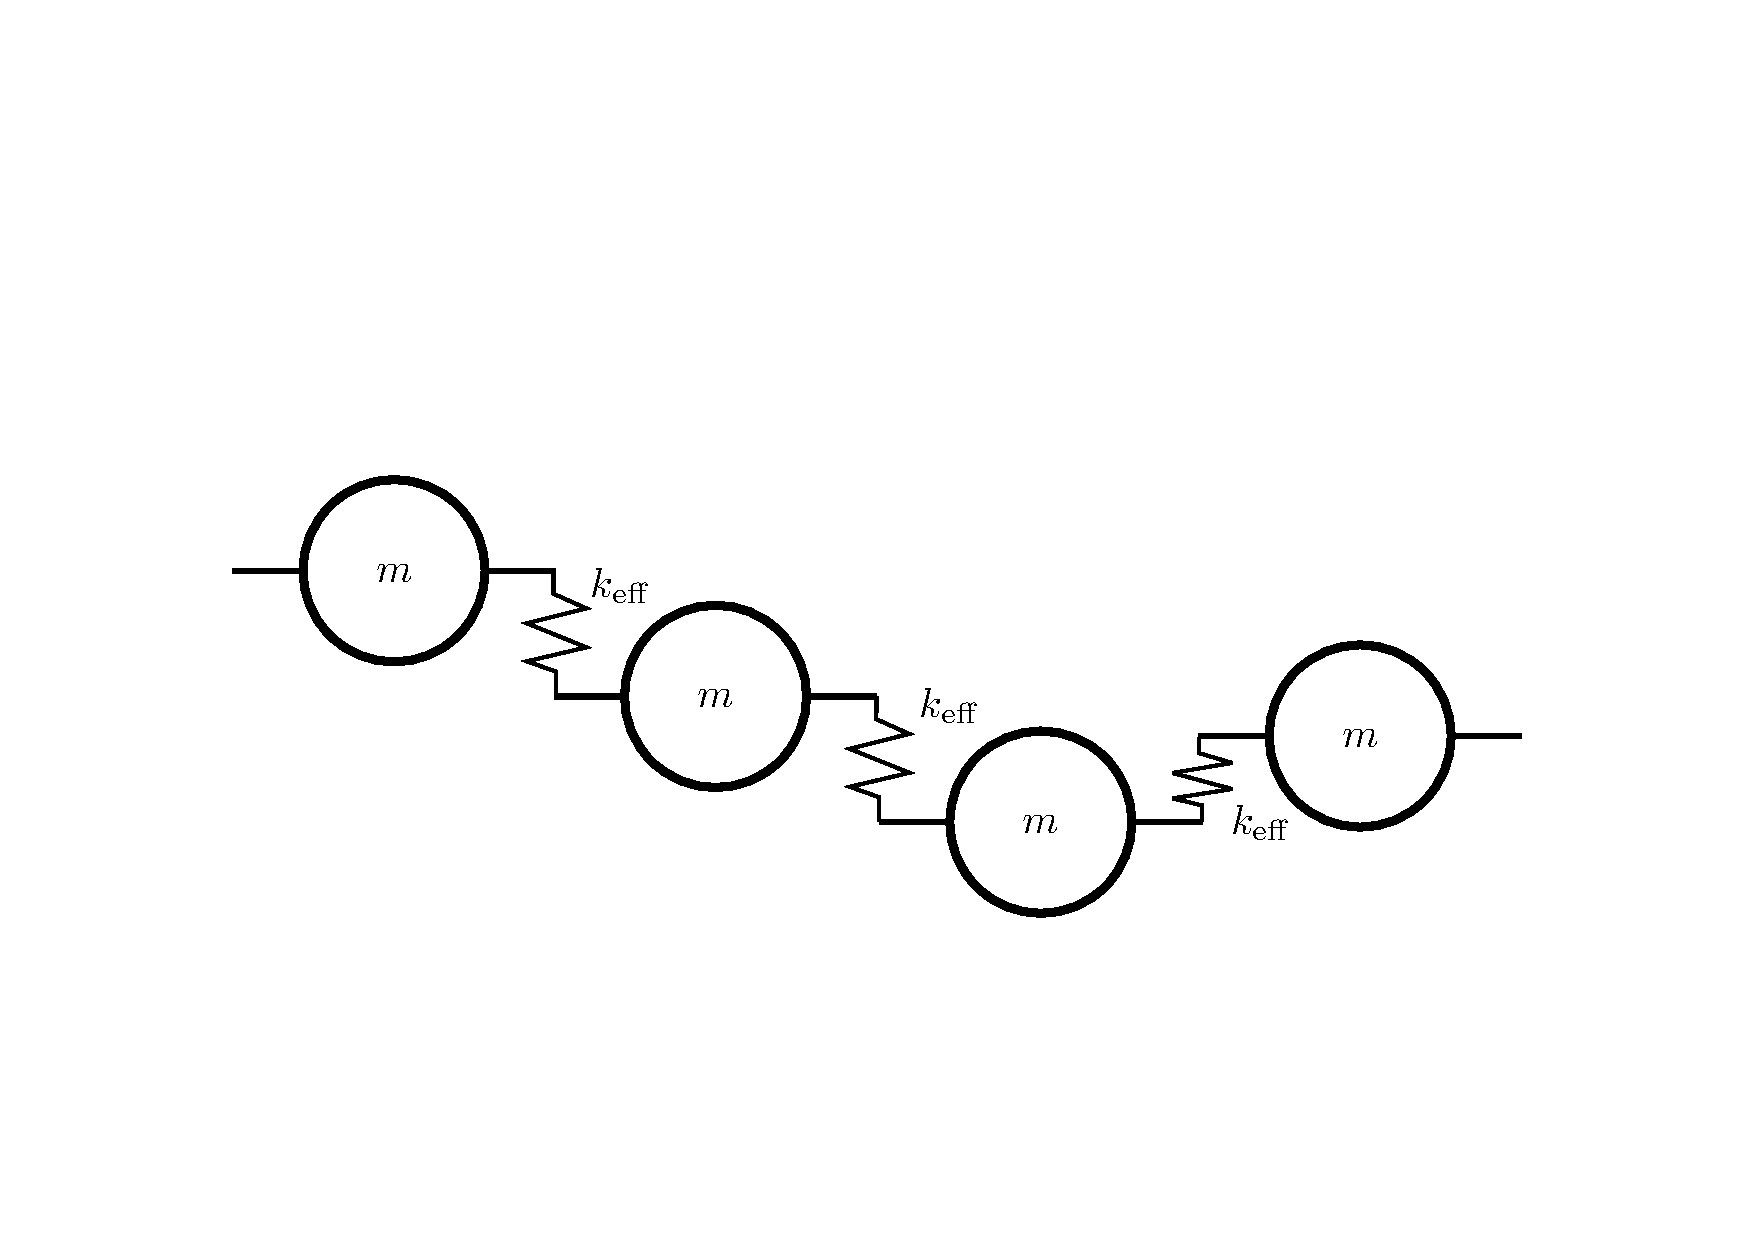
\includegraphics[width =.5\textwidth]{results/equivalance.pdf}
  \caption{Mapping of the actual configuration of the wave machine with the rotating levers to a configuration where the individual masses are coupled in the vertical direction by springs.}\label{fig:equivalence}
\end{figure}
I therefore had to map the more complicated experimental situation to the  scheme depicted in Figure \ref{fig:equivalence}. There the wave is still transverse but the described theory above remains valid. To do this mapping, I have to convert the spring constant in the current experiments into the spring constants which can be used in this simplified model. I analyse the equation of motion for the levers under the torque of the springs based on the sketch in Figure \ref{fig:config}. The torque acting on the levers in Figure \ref{fig:config} is given by the springs with the spring constant $k_s$. Changing the angle by an amount $\theta$ extends the spring by $l_{1}\sin(\theta)$ such that the force of the spring on one side is $k_s\, l_{1}\sin(\theta)$. This force is applied on a lever with a length $l_{1}\cos(\theta)$. The torque is acting twice due to the two springs, one on each side of the lever. I abbreviate $k=2k_{s}$. The motion of the lever is determined by the angular acceleration $\ddot{\theta}$ and the moment of inertia of a dumbbell $I=2 m l_{2}^2$. Thus the equation of motion reads
\begin{equation}\label{eq:eqofmotion}
    I\ddot{\theta}=-k\, l_{1}\sin(\theta)\, l_{1}\cos(\theta)
\end{equation}
which can be transformed into 
\begin{equation}
    \ddot{\theta}=-\frac{k\, l_{1}^2}{2m\,l_{2}^2}\sin(\theta)\,\cos(\theta)
\end{equation}
If I further assume that all angles $\theta$ are small, I can approximate $\sin(\theta)\approx \theta$ and $\cos(\theta)\approx 1$. Accordingly I can simplify the equation of motion by
\begin{equation}
    \ddot{\theta}=-\frac{k\, l_{1}^2}{2m\,l_{2}^2}\theta
\end{equation}
which is the standard differential equation of an harmonic oscillator, where the factor in front of $\theta$ resembles the square of the resonance frequency. 
I readily obtain
\begin{equation}
    \omega_{0}^{2}=\frac{k\, l_{1}^2}{2m\,l_{2}^2}
\end{equation}
Following the definition of the spring constant of the simple harmonic oscillator, I can define an effective spring constant for the replacement model of
\begin{equation}
    k_{\rm eff}=k\frac{l_{1}^2}{2l_{2}^2}=m\omega_{0}^2
\end{equation}
Using this effective spring constant and the mass $m$ I can map the coupled lever oscillators to the situation described in the theory and Fig. \ref{fig:equivalence}. In the case of a chain of oscillators with an internal oscillator, the value of $m$ has to be replaced by $M_{\rm eff}$.

However, the case for the internal oscillator is slightly different as the the torque is acting four times due to the four spring, two on each side of the lever. I therefore modify eq. \ref{eq:eqofmotion} to this specific case which yields
\begin{equation}
    I\ddot{\theta}=-2k\, l_{1}\sin(\theta)\, l_{1}\cos(\theta)
\end{equation}
By performing similar steps as illustrated above I obtain the effective spring constant for the internal oscillator.
\begin{equation}
    k^{\rm int}_{\rm eff}=k\frac{l_{1}^2}{l_{2}^2}=m\omega_{0}^2
\end{equation}
The effective spring constant $k_{\rm eff}$ can be determined from the experiments when the mass at the end of the lever $m$ is known. If further the two lengths $l_{1}=2\, {\rm cm}$ and $l_{2}=10.5\, {\rm cm}$ are inserted, I can determine the spring constant of the springs in the lever setup, which has also been measured with a force sensor to be $k_{s}=32.3\, {\rm N/m}$.


\subsection{Single mass with an internal oscillator}
I first study the properties of a single oscillator (configuration C1, see section \ref{sec:section3}). I examine the amplitude ratio between the two masses $M_0$ and $m$ and the phase angle between their oscillation. The experiment was conducted in the range from $f=2.70$ Hz to $f=3.20$ Hz at increments of 0.05 Hz in 11 measurements. 
\begin{figure}[hbt]
  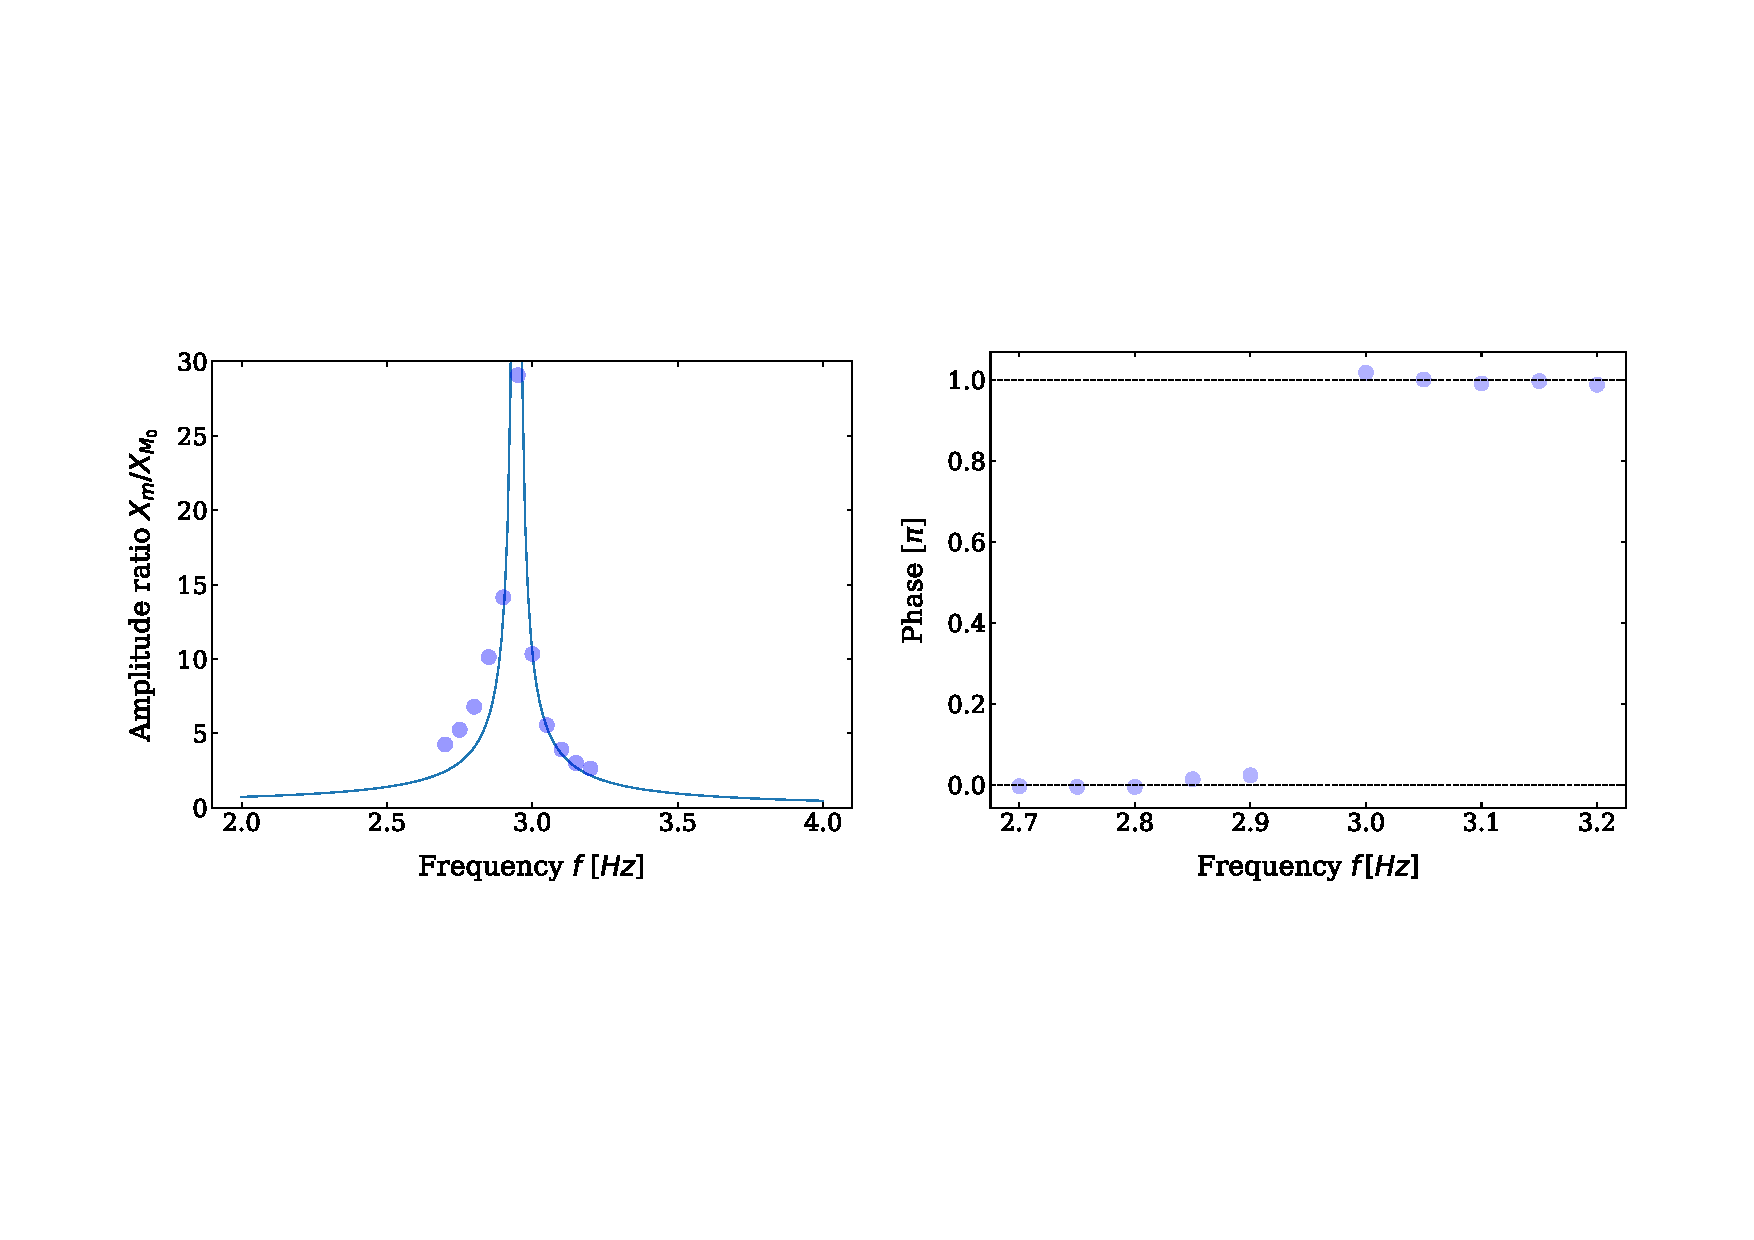
\includegraphics[width=0.9\columnwidth]{results/condition3_amplitude_ratio}
  \caption{(left) Amplitude ratio $|X_m|/|X_{M_0}|$ between $m$ and $M_0$ of a single oscillator (configuration C1) under periodic excitation. The solid line is obtained from eq. \ref{eq:ratio} inserting the experimental data on mass and $k_{\rm eff}$. (right) Phase difference between the excitation frequency (measured at $M_{0}$) and the observed oscillation of $m$.} \label{fig:figure17}
\end{figure}
Figure~\ref{fig:figure17} displays the amplitude ratio between the free lever and the excited  lever $X_{m}/X_{M_{0}}$. The amplitude of $m$ enlarges until a frequency of $f_{0}=2.945 \:Hz$ corresponding to eq.~\ref{eq:ratio}. This frequency is the resonance frequency of the oscillator. The amplitude ratio is maximum at this frequency and decays to lower and higher frequencies. At frequencies larger than the resonance frequency, $m$  moves in the opposite direction with respect to $M_0$ (phase angle of $\pi$, right plot in Fig. \ref{fig:figure17}). 

\subsection{Simple chain of masses}
In configuration C2 (chain of coupled oscillators) I investigated the transmission $|X_{21}|/|X_1|$ of the system at different excitation frequencies. In the frequency range from $f=0.9$ Hz to $f=2.0$ Hz, I recorded the amplitude with a frequency increment of 0.02 Hz in 56 individual measurements. In the range from $f=2.2$ Hz to $f=4.0$ Hz I took measurements every 0.2 Hz (10 measurements). From $f=4.1$ Hz to $f=4.5$ Hz additional 5 measurements were conducted at increments of 0.1 Hz. The experimental results for the transmission are shown in Figure \ref{fig:figure19}.
\begin{figure}[hbt]	
  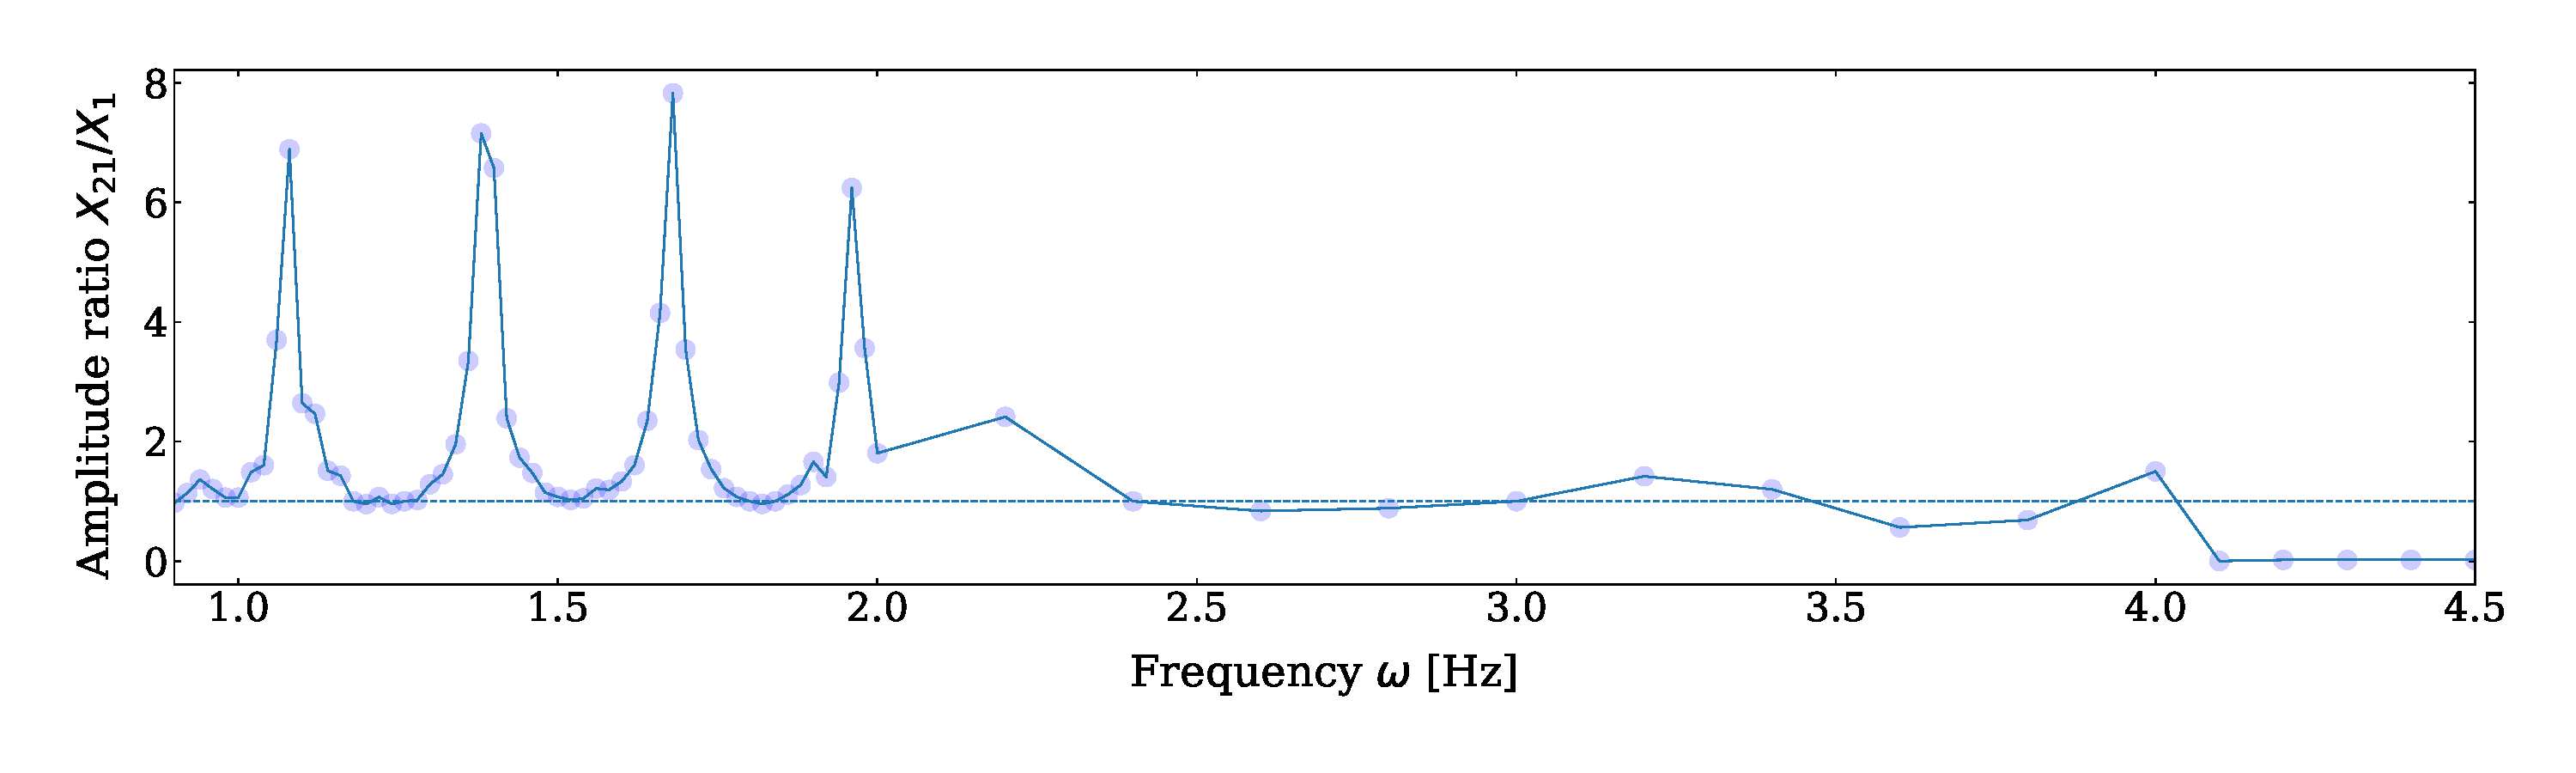
\includegraphics[width=\columnwidth]{results/condition1_amplitude}
  \caption{Amplitude ratio $|X_{21}|/|X_1|$ between the first and last lever of the wave machine under harmonic excitation (configuration C2). The dotted line represents the amplitude ratio of  $|X_{21}|/|X_1|=1$}\label{fig:figure19}
\end{figure}
The graph shows four resonances at $f=1.08$ Hz, $f=1.39$ Hz, $f=1.68$ Hz, $f=1.96$ Hz, where the displacement $X_{21}$ is enhanced by a factor of more than 6. These resonances occur due to the finite length of the chain, which supports a discrete number of standing waves where an integer multiple of half the wavelength fits on the chain. An overall number of 11 resonances should be visible. In the range from $f=2.2$ Hz to $f=4.5$ Hz, the individual peaks in this region are unresolved due to the lower frequency resolution. Beyond $f=4.1$ Hz the amplitude ratio drops to zero due to the fact that the experiment was conducted with oscillators at discrete distances of $a=2\,{\rm cm}$. As the frequency of wave increases its wavelength decreases. The cut-off frequency displayed in Figure \ref{fig:figure19} corresponds to the frequency at which the shortest wavelength ($\lambda=2 a=4$) is realized by the levers, i.e. where neighbouring levers are elongated in opposite directions.

As described in the theory section, the wave propagation along a periodic chain is characterized by the dispersion relation

\begin{figure}[hbt]
  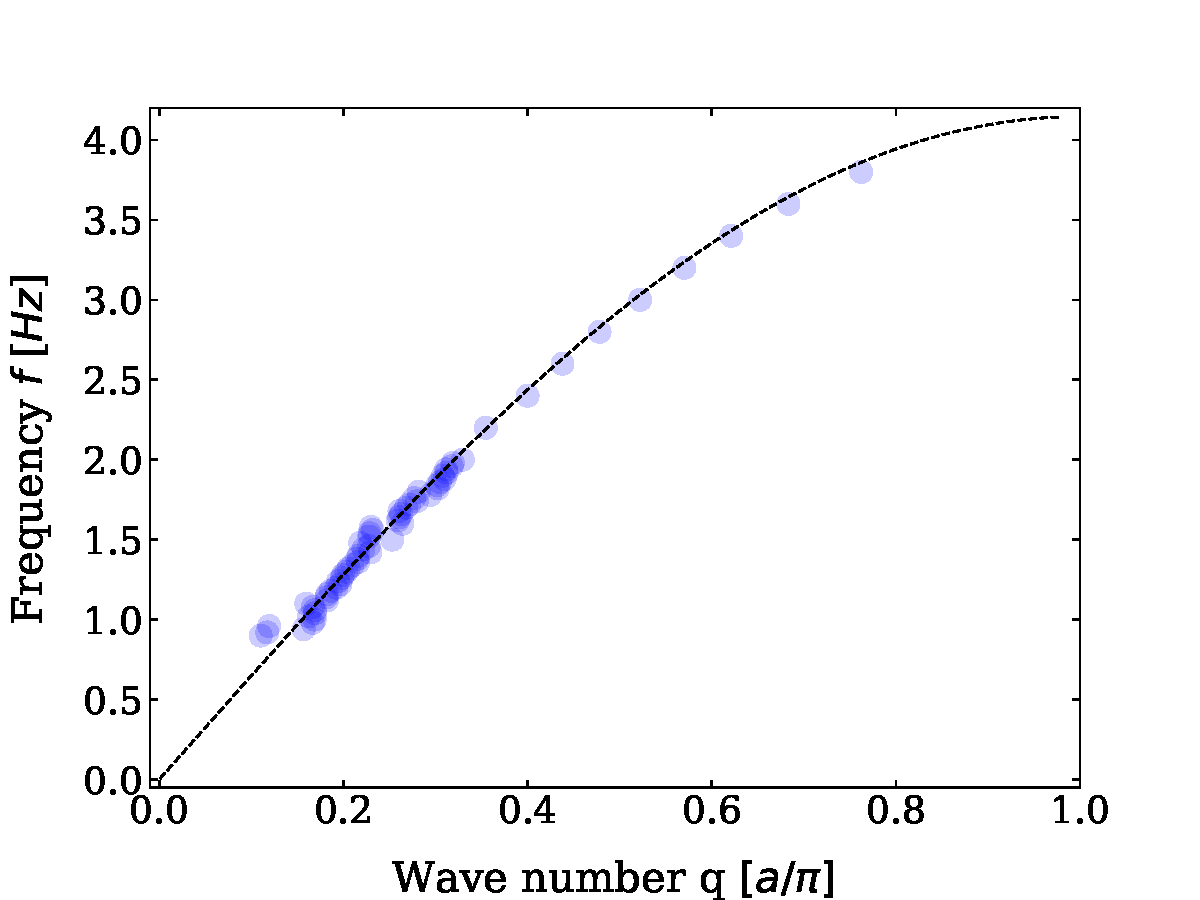
\includegraphics[width=0.5\columnwidth]{results/dispersion_simple_chain.pdf}
  \caption{The dispersion relation $f(q)$ of the wave machine as derived from the experimental results. The wavenumber is given in units of $a/\pi$, where $a$ is the distance between neighbouring levers. The dashed lines represents the theoretical prediction (eq. \ref{eq:25}) using the effective spring constant $k_{\rm eff}$, $a=2\,{\rm cm}$ and $m=7.3\, {\rm g}$.}\label{fig:figure18}
\end{figure}
 
 Figure \ref{fig:figure18} displays a plot of the frequency $f$ of the excitation and the connected wavenumber $q$ in units of $a/\pi$. $a/\pi=1$ is corresponding to the wavelength $\lambda=2a$, which is the shortest possible wavelength on the chain observed at a frequency of $f=4.1$ Hz. The same graph also shows the theoretically predicted dispersion relation for the present system according to eq. \ref{eq:25} using $M_{\rm eff}=m=7.3$ g and $k=k_{\rm eff}$. 
 
 Overall, the chain of coupled oscillators provides results which nicely agree with the theoretical predictions. The chain supports waves in a well defined frequency range, with a cut-off frequency that corresponds to the shortest possible wavelength in the system due to the finite number of oscillators. The observed discrete resonances are the result of the finite length of the chain, that causes resonances at specific frequencies that correspond to standing waves on the chain.
 
\subsection{Chain of masses with an internal oscillator}
The dispersion relation and also the transmission of the chain is modified when inserting the brackets and providing an internal oscillator to each oscillator mass. An excitation may thus yield a localised oscillation of an internal oscillator without a propagation of a wave.

To identify the changes, I have modified the wave machine with 7 brackets and measured the amplitude of the levers as a function of frequency in the frequency range between $f=$ 1.8 Hz to $f=$ 4.4 Hz with a frequency increment of 0.1 Hz (overall 27 movies).
The results are summarized in Figure \ref{fig:figure20}. The left part of the plot displays the dispersion relation, while the right part depicts the transmission of the system. Note that due to the brackets the individual oscillators of the chain are now spaced at $a=$ 6 cm, while the simple chain had a spacing of $a=$ 2 cm. 
\begin{figure}[hbt]
  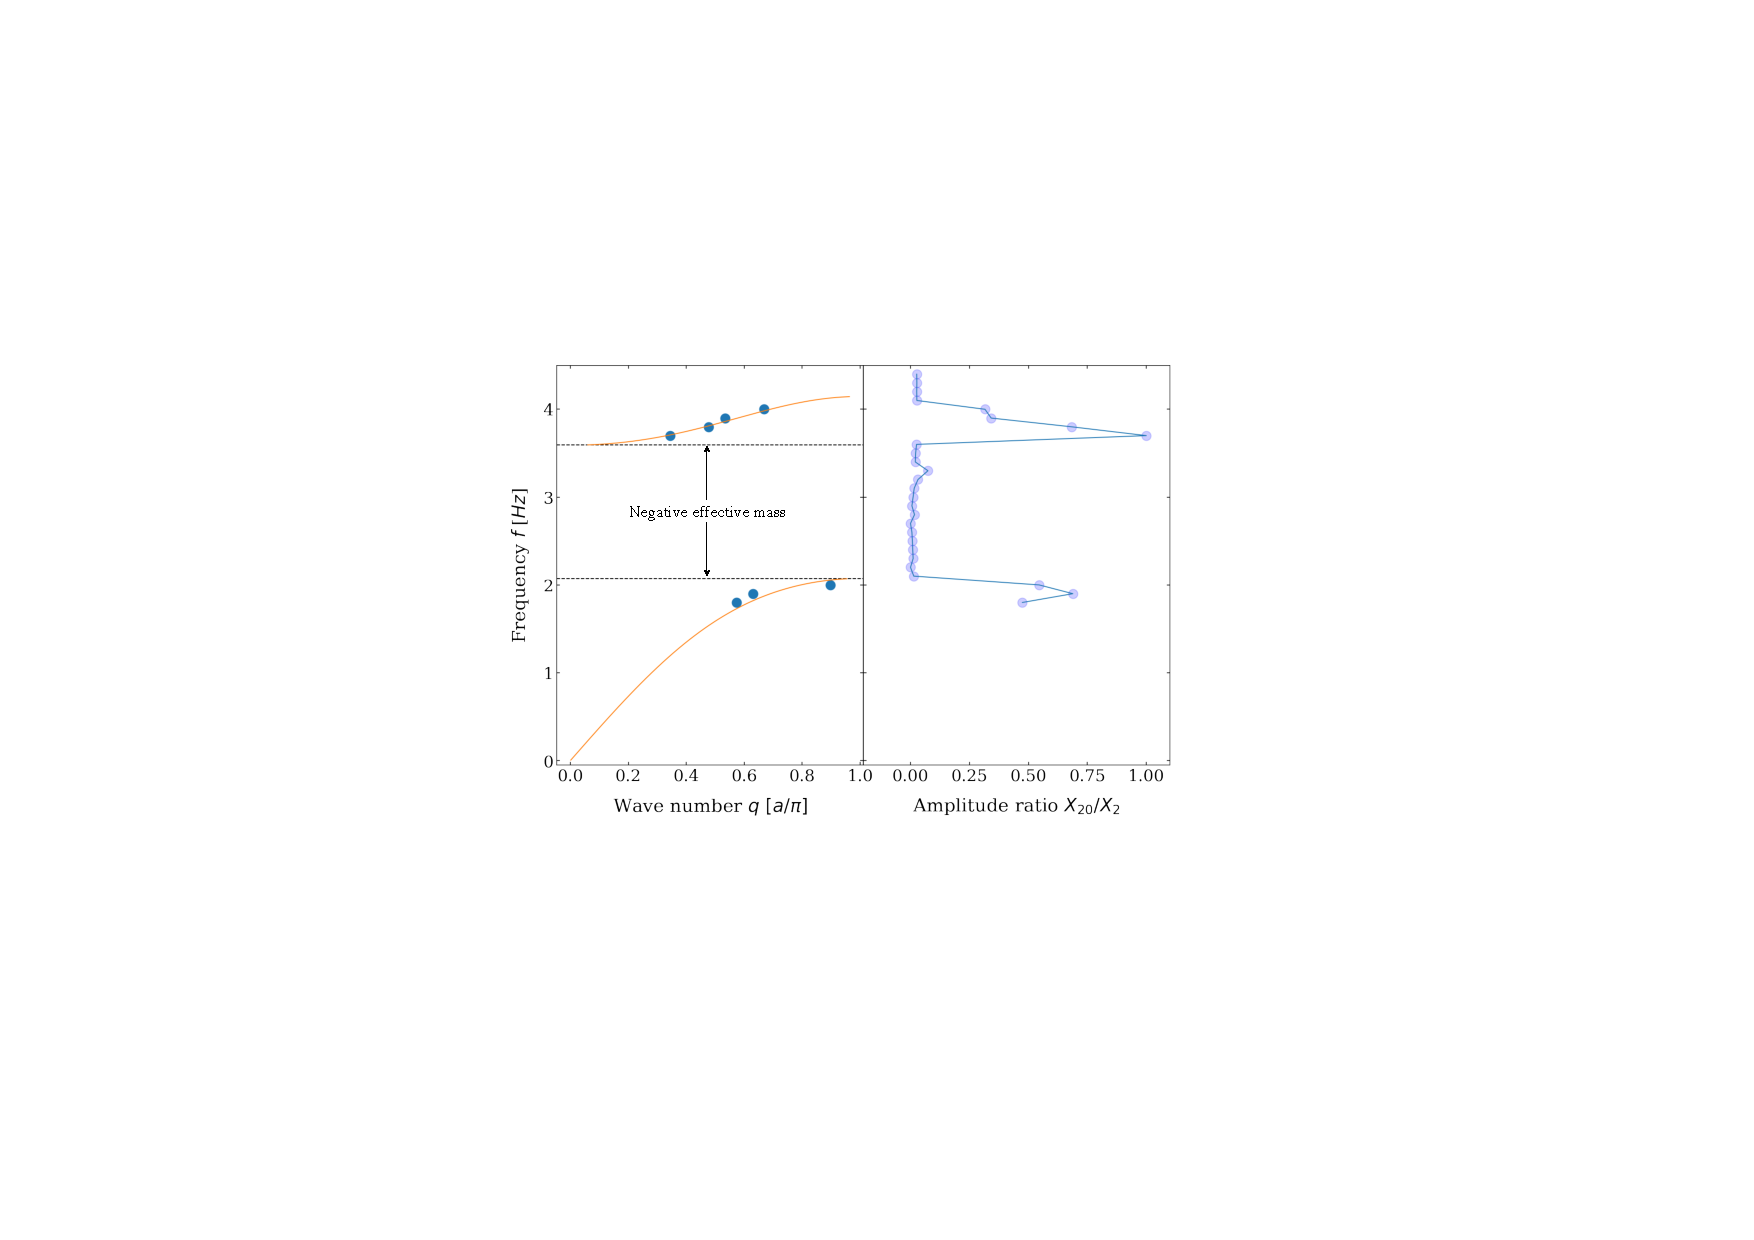
\includegraphics[width=.7\columnwidth]{results/condition3_dispersion_transmission.pdf}
  \caption{(left) Dispersion relation for the coupled masses with internal oscillators in configuration C3. The dots show the experimental results. The lines are the theoretical predictions with the frequency dependent effective mass $M_{\rm eff}$ (eq. \ref{eq:20}), $a=6$ cm and $k=1.24$ N/m. (right) The transmission of the chain $X_{20}/X_{2}$ as a function of frequency.}\label{fig:figure20}
\end{figure}
In the frequency range between $f=2.1$ Hz and $f=3.6$ Hz no wave propagation is supported by the chain (Fig. \ref{fig:figure20} right). Wave propagation is, however, possible at frequencies below $f=2$ Hz and between $f=3.6$ Hz and $f=4.1$ Hz. This gap in the dispersion relation is a clear sign of the introduced internal oscillators. This frequency range corresponds to the negative effective mass of the individual units with the internal oscillators and therefore proofs my hypothesis, that such a negative effective mass becomes visible in a band gap of a modified chain of oscillators. Note that the second band starting at $f=3.6$ Hz at $q=0$ yields a point where the wavelength is infinity despite a non-zero frequency. This means all lever arms oscillate in phase and the effective mass is zero. 

The experimental values of the dispersion relation is compared to the theoretical prediction eq. 27, which is shown in the Figure \ref{fig:figure20} by the yellow line. The theoretical prediction fits perfectly to the experimental observation. While the experimental data in the dispersion relation are only a few points, the band gap is clearly visible from the transmission.

Since within the band gap there is no propagation of the wave possible, the excitation of the oscillators only yields so called evanescent waves. This means that the amplitude of the local oscillations of the oscillators is decaying exponentially as described in section \ref{sec:coupled:waves}. This is also nicely reflected by Figure \ref{fig:figure21}.
\begin{figure}[hbt] 
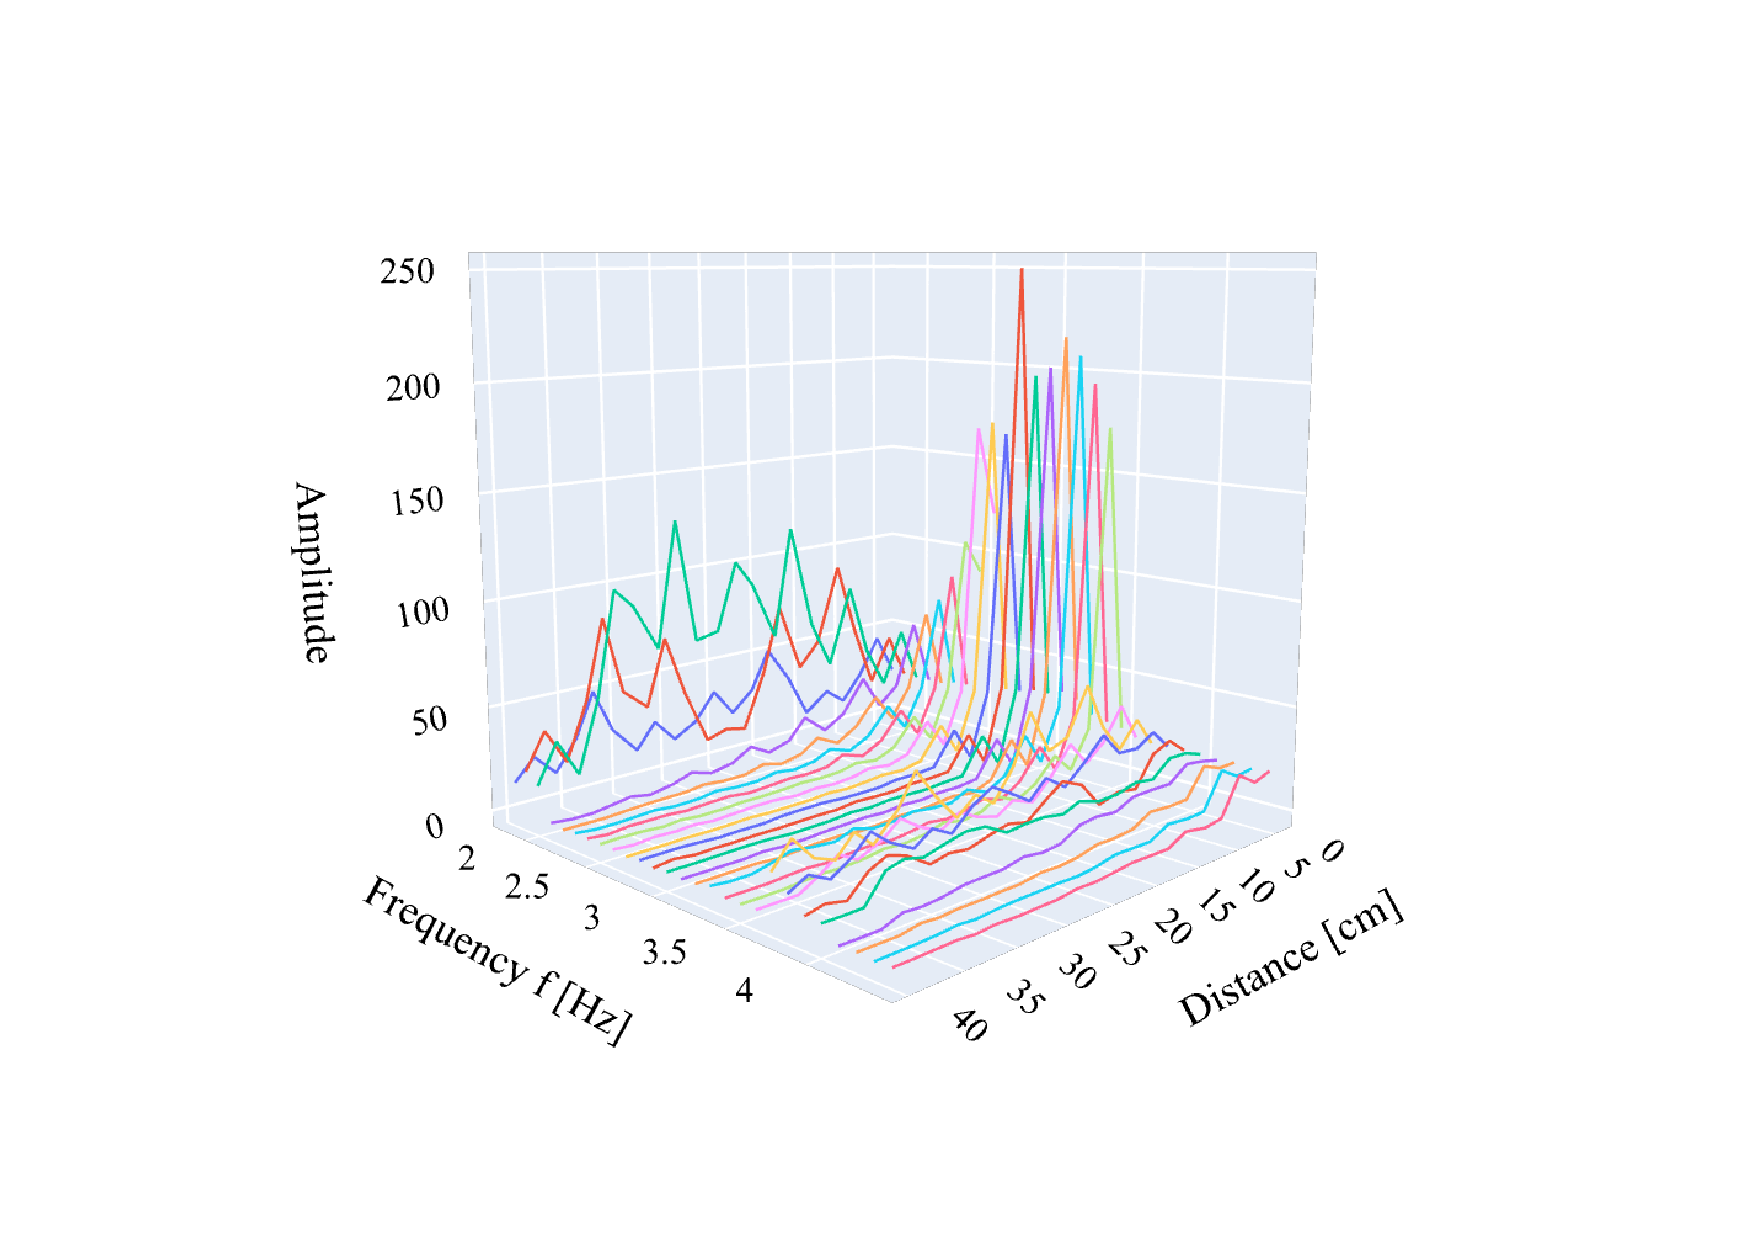
\includegraphics[width=.8\textwidth]{results/evanescent.pdf}
\caption{Plot of all the maximum amplitudes of all lever arms from all frames  as a function of the lever arm position and the frequency for the configuration C3 with a hidden oscillator. The amplitude is given in arbitrary units. }\label{fig:figure21}
\end{figure}

\section{Conclusion}
In my experiments and theoretical considerations I have researched the question if I can create an effective negative mass by designing an oscillator with a hidden internal oscillator. When arranging these hidden oscillators into a chain and coupling them by springs, the negative effective mass becomes visible in the so-called dispersion-relation by a band gap, i.e. a frequency region, where waves are unable to propagate in the chain. 
Using a wave machine of coupled lever arms and a modification by 3D printed brackets I have been experimentally able to create a system with a negative effective mass and observe exactly the hypothesised band gap. I have further adopted the experimental situation to comply with a theory that was available from the literature. This allows me to do theoretical predictions to my experimental observation. I found that all experimental observation are well matched with the theoretical predictions. Thus my hypothesis is validated by my experiments. 
As an outlook, I would like to mention that more extended measurements on the dispersion relation of the modified wave machine may yield seven more data points in the dispersion relation. Such measurements are, however, very time consuming and could not be carried out by me during the available amount of time.
\clearpage
\section{References}
\begin{enumerate}
\item{“English Dictionary, Thesaurus, \& Grammar Help.” Lexico Dictionaries | English, Lexico Dictionaries, 2019, www.lexico.com/en.}
\item{Föll, H. “Effective Masses.” 2.3.1 Effective Masses, 2004, www.tf.uni-kiel.de/matwis/\\amat/semi\_en/kap\_2/backbone/r2\_3\_1.html.}
\item{“II.8. Reflection, Transmission and Absorption.” Reflection, Transmission, and Absorption, 2008, light-measurement.com/reflection-absorption/.}
\item{Shanshan Yao et al 2008 New J. Phys. 10 043020}
\item{Stéfan van der Walt, Johannes L. Schönberger, Juan Nunez-Iglesias, François Boulogne, Joshua D. Warner, Neil Yager, Emmanuelle Gouillart, Tony Yu and the scikit-image contributors. scikit-image: Image processing in Python. PeerJ 2:e453 (2014) https://doi.org/10.7717/peerj.453}
\item{Winter, Rudi. “Condensed Matter Physics.” Dispersion Relations :: Condensed Matter Physics :: Rudi Winter's Web Space, 15 Dec. 2018, users.aber.ac.uk/ruw/teach\\/334/disprel.php.}
\end{enumerate}
\clearpage
\section{Appendix}
\begin{figure*}[hbt]
	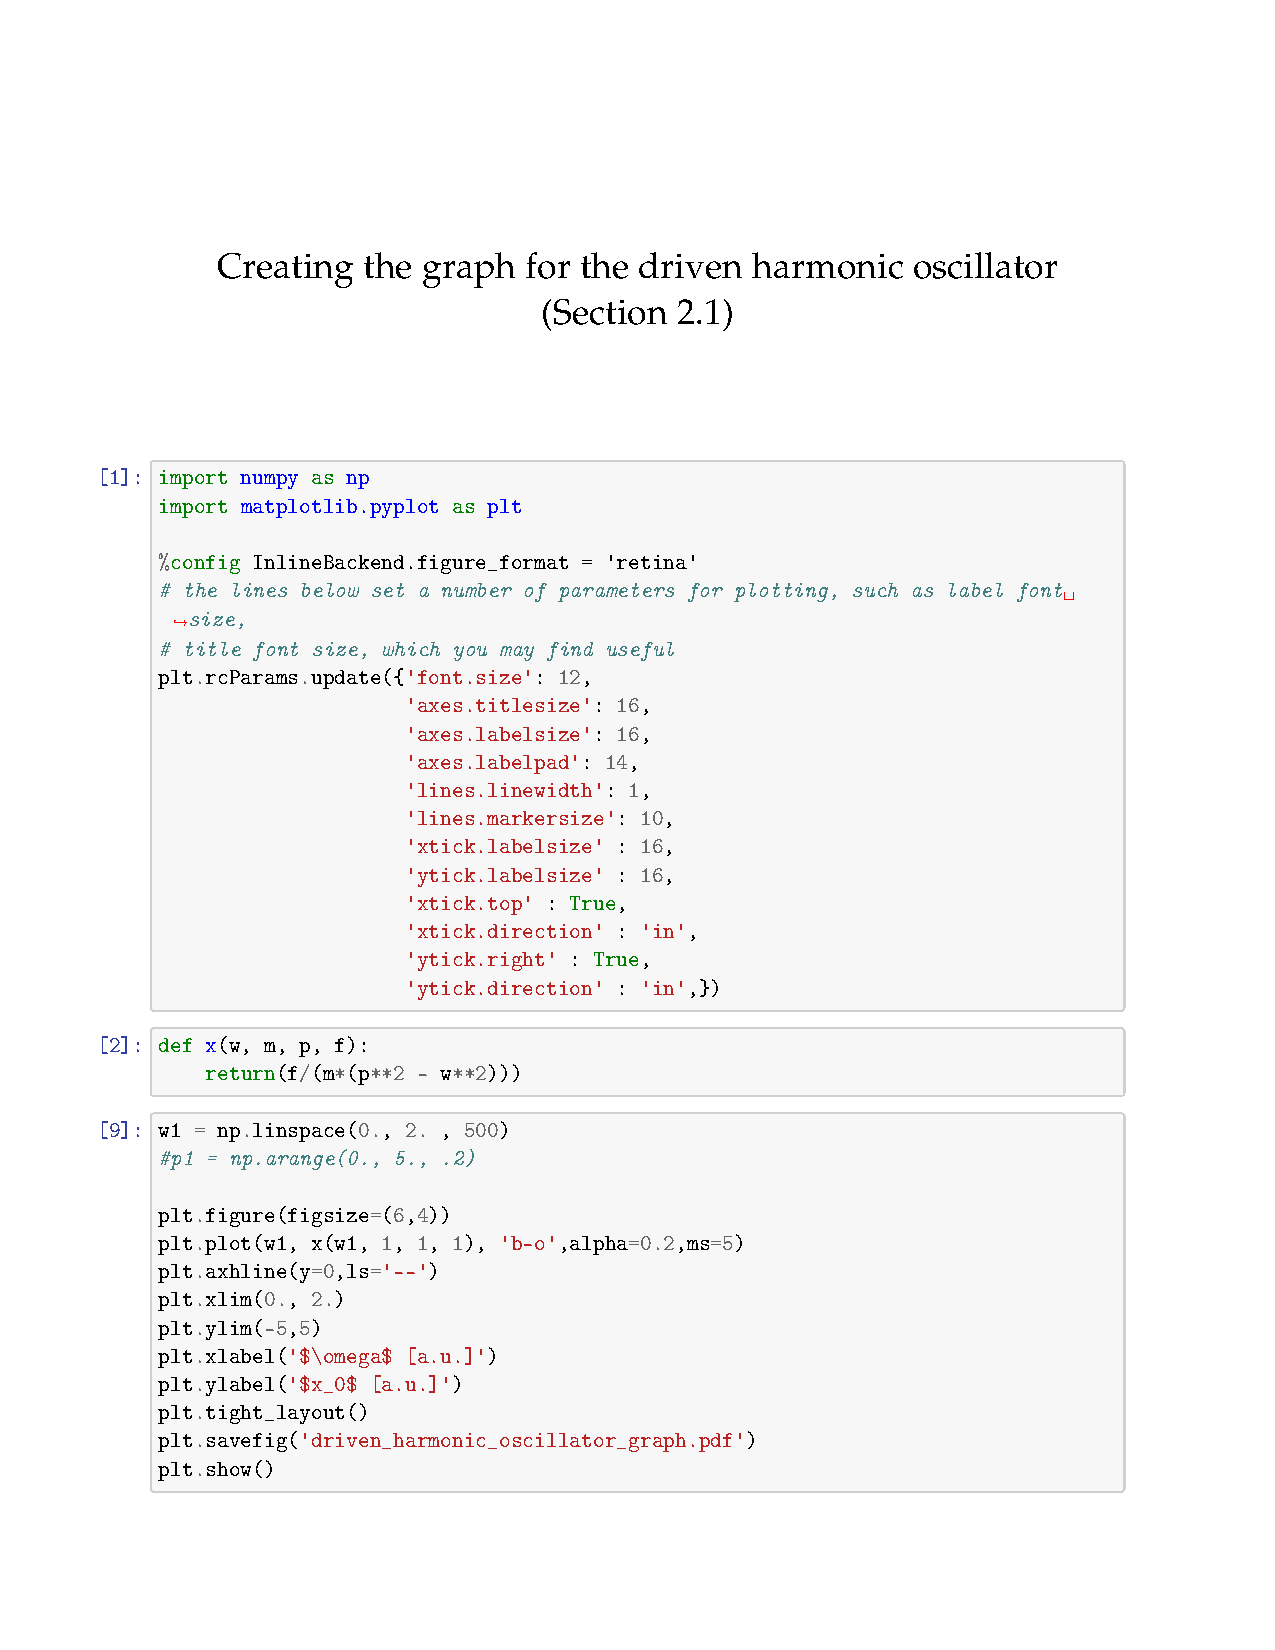
\includegraphics[width=.96\textwidth]{code/python_code_c4.pdf}
\end{figure*}
\clearpage
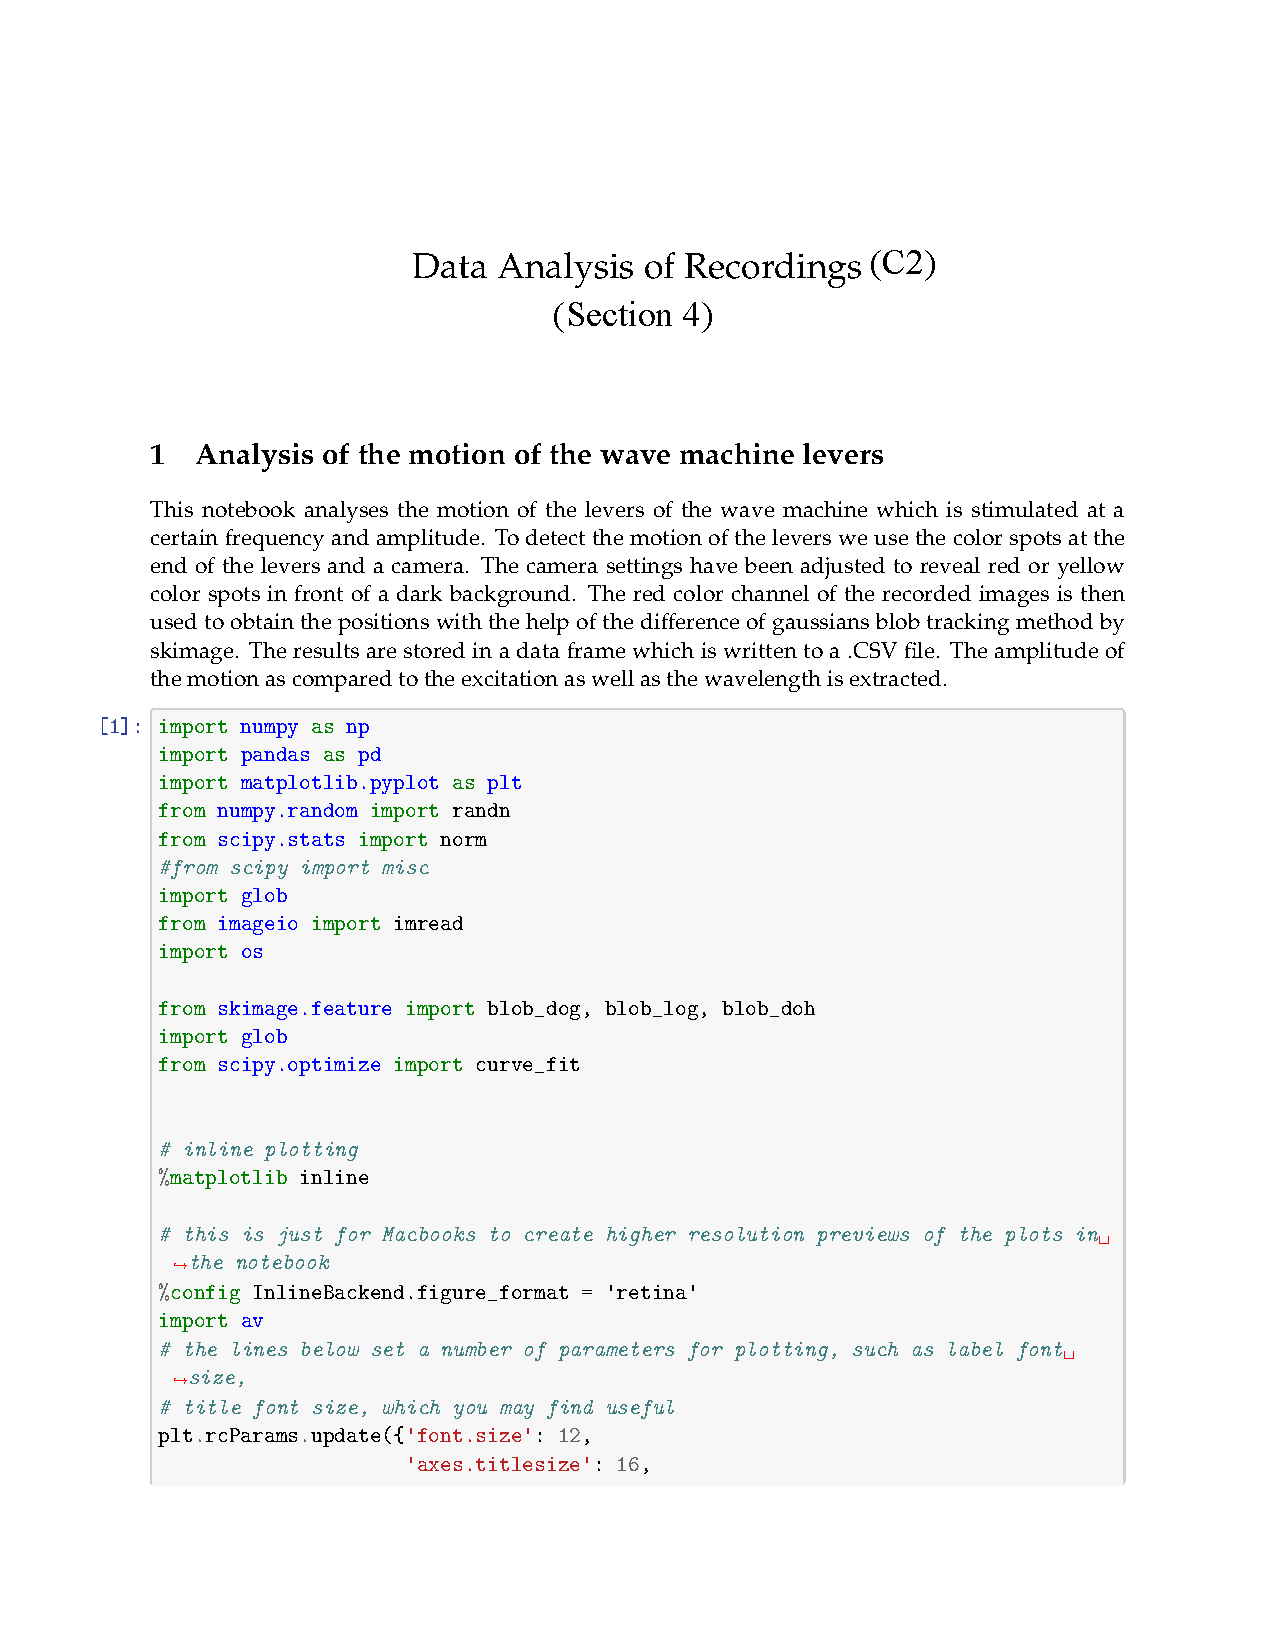
\includepdf[pages=-]{code/python_code_c2.pdf}
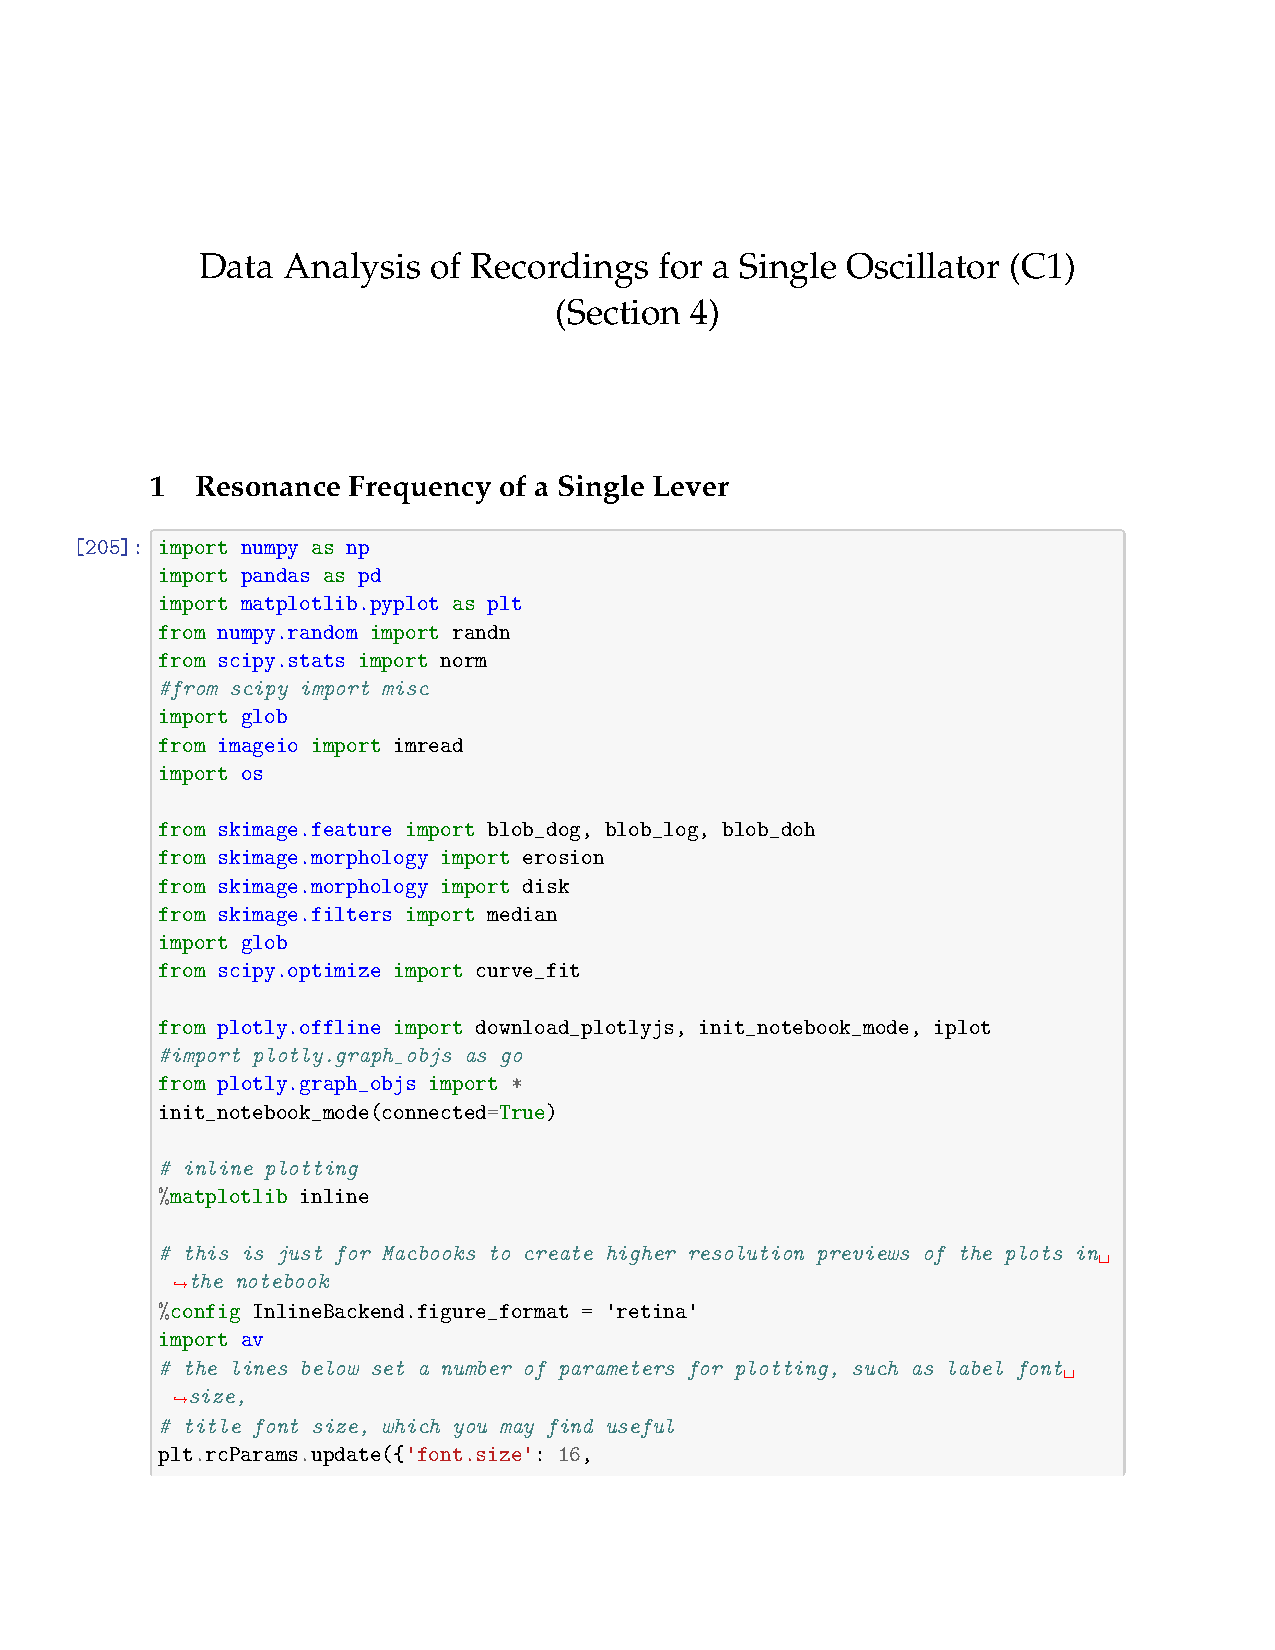
\includepdf[pages=-]{code/python_code_c1.pdf}
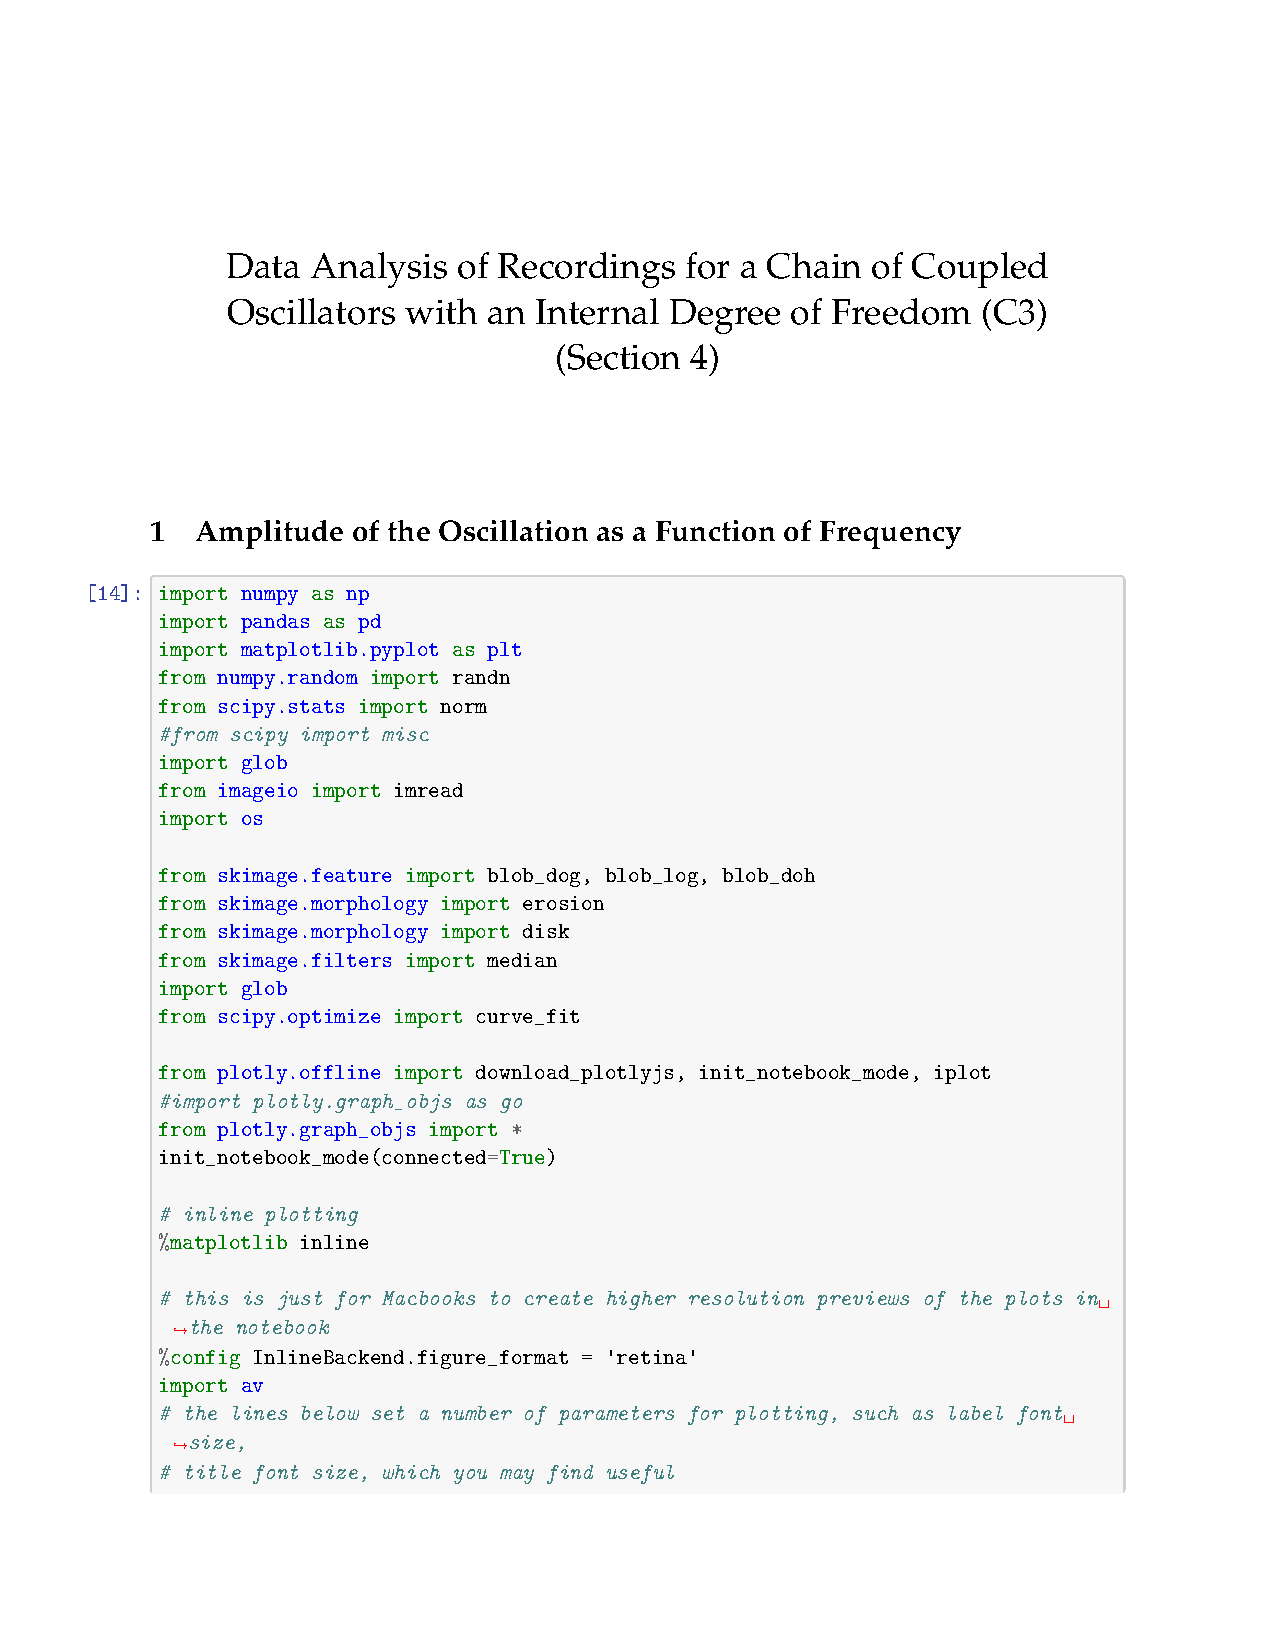
\includepdf[pages=-]{code/python_code_c3.pdf}


\end{document}
